\documentclass{MSthesis} 
% subclass of the document class report.
\pgfplotsset{compat=1.16}

\begin{document}

% Formatting titles and spaces 

% Originally its
% Chapter 1:
% Name of chapter one
\titleformat{\chapter}[hang] 
{\normalfont\huge\bfseries}{\thechapter}{1em}{}  

% left margin, vertical space,  space to section, 
\titlespacing*{\chapter}{0cm}{0cm}{0cm}
\titlespacing*{\section}{0cm}{0cm}{0cm}
\titlespacing*{\subsection}{0cm}{0cm}{0cm}
\titlespacing*{\subsubsection}{0cm}{0cm}{0cm}
%%%%%%%%%%%%%%%%%%%%%%%%%%%%%%%%%%%%%%%%%%%%%%%%

% USING THE TWOSIDED OPTION left = inner , and right = outer
\myfrontpage
\mycopyright

%\newpage\null\thispagestyle{empty}\newpage

% Abstract should have first page nr,
\pagenumbering{roman}
\chapter*{Abstract}
\addcontentsline{toc}{chapter}{Abstract}


%\begin{itemize}
%    \item Introduce topic and why its important
%    \item Introduce a challenge or unresolved issue that you will try and solve
%    \item What have you done to try and solving this
%    \item Main result - Include the numerical result of your best model
%    \item The implications in the context of 1+2
%\end{itemize}

Increased anthropogenic emissions of nitrogen oxides, carbon monoxide, volatile organic compounds and methane causes production of ozone in the troposphere, particularly in the northern hemisphere. This causes warming of the northern hemisphere troposphere as tropospheric ozone acts as a greenhouse gas. Ozone depletion events (ODEs) caused by reactive halogens in the Arctic are a well known and thoroughly studied phenomena, which may modulate the warming effect of tropospheric ozone in the Arctic. The purpose of this thesis is to develop a reliable halogen-chemistry scheme in the Oslo CTM3 and estimate performance of the new scheme by comparing with observations and the original CTM3. The ozone-induced radiative forcing (RF) due to the implemented halogen chemistry can then be estimated. The new scheme was run for 2001 and 2013, but only the 2001 run was compared with observations. The new scheme shows no significant correlation with ground-based measurements of ozone. In the new scheme, \chem{HBr} appears to be the dominant halogen species during and after ODEs. The halogen-induced ozone depletion in the new scheme works, but it causes too much ozone depletion. Diverging results in the 2001- and 2013-run makes it impossible to conclude any horizontal or vertical dependence regarding tropospheric ozone-induced RF with regards to the new halogen implementation. The temporally (February to June) and globally averaged RF due to tropospheric ozone yielded by the BE-branch demonstrates large deviations between the 2001-run, RF $=-0.012\pm0.12$ Wm$^{-2}$, and the 2013-run, RF $= 0.45\pm0.42$ Wm$^{-2}$. Due to the inconsistency in RF and the fact that the present-day and pre-industrial setup of the BE-branch, these estimates are not correct. The new scheme does not sufficiently reproduce the observed ODEs in the Arctic, and the RF-estimates are variable and inconsistent. Further development of the halogen chemistry is needed to estimate the effect on ozone-induced RF in the troposphere. 
\cleardoublepage



\chapter*{Acknowledgement}
\addcontentsline{toc}{chapter}{Acknowledgement}
%I would first and foremost like to thank my main supervisor Terje, for always having a couple of minutes when all seems desperate. Your theoretical support and discussions has been extremely appreciated. A big thanks to Stefanie as well for answering patiently to big and small questions and bringing order to overwhelming chaos. Marianne

%\medskip

%Mamma, pappa and Elisabeth deserves a gold medal for always providing a safe space in frustrating times and for still wanting to be my family. Your moral support has been invaluable throughout these years, and I love you all very much!

%\medskip

%Lastly, but no less, I would like to thank Johanne, Ingvild, Hanne, Hanna, Hanna and Inger Johanne for being the best friends anyone could ask for. You are there when I need to sing and dance, run, drink wine or laugh, and have made my life a great deal easier. 

\cleardoublepage

\tableofcontents

% Clear double page --> New chapters or listings begin on odd numbered pages.
\cleardoublepage

\listoffigures
\addcontentsline{toc}{chapter}{\listfigurename}
\cleardoublepage

% List of tables 
\listoftables
\addcontentsline{toc}{chapter}{\listtablename} % add list of tables to contents line
\cleardoublepage

% List of acronyms
\printglossary[type=\acronymtype]
\addcontentsline{toc}{chapter}{Acronyms}

% Example acronyms list.
% Adding seasons to the acronyms list.
\newacronym{mam}{MAM}{March April May}
\newacronym{djf}{DJF}{December January February}
\newacronym{jja}{JJA}{June July August}
\newacronym{son}{SON}{September October November}
\newacronym{eu}{EUR}{Europa}

% Radiation 
\newacronym{nir}{NIR}{Near-Infrared}
\newacronym{swir}{SWIR}{Short-Wavelength infrared}
\newacronym{mw}{MW}{Mid-Wavelength infrared}
\newacronym{lwir}{LWIR}{Long-Wavelength infrared}

%%%%%%%%%%%%%%%%%%%%%%%%%%%%%%%% MET 
\newacronym{bams}{BAMS}{Bulletin American Meteorological Society}
\newacronym{seviri}{SEVIRI}{Spinning Enhanced Visible and Infrared Imaging}
\newacronym{msg}{MSG}{METeosat Second Generation}
\newacronym{ecmwf}{ECMWF}{European Centre for Medium-Range Weather Forecasts}
\newacronym{eumetsat}{EUMETSAT}{European Organisation for the Exploitation of Meteorological Satellites}
\newacronym{esa}{ESA}{European Space Agency}
\newacronym{ecc}{ECC}{European Cloud Cover}
\newacronym{ccn}{CCN}{cloud condensation nuclei}
\newacronym{inp}{INP}{ice nuclei particle}
\newacronym{cre}{CRE}{cloud radiative effect}
\newacronym{ghg}{GHG}{green house gases}
\newacronym{ipcc}{IPCC}{intergovernmental panel of climate change}
\newacronym{toa}{TOA}{top of the atmosphere}
\newacronym{ecs}{ECS}{equilibrium climate sensitivity}
\newacronym{cmip5}{CMIP5}{the coupled model intercomparison project phase 5}
\newacronym{cmip6}{CMIP6}{the coupled model intercomparison project phase 6}
\newacronym{ppm}{ppm}{parts per million}
\newacronym{rcp}{RCP}{representative concentration pathways}
\newacronym{ssp}{SSP}{shared socioeconomic pathways}
\newacronym{pdf}{PDF}{probability density function}
\newacronym{gcm}{GCM}{general circulation model}
\newacronym{esm}{ESM}{Earth system model}
\newacronym{calipso}{CALIPSO}{Cloud-Aerosol Lidar and Infrared Pathfinder Satellite Observations}
\newacronym{modis}{MODIS}{Moderate Resolution Imaging Spectroradiometer}
\newacronym{json}{JSON}{Java Script Object Notification}
\newacronym{netcdf}{netCDF}{network Common Data Form}
\newacronym{grib}{GRIB}{GRIdded Binary or General Regularly-distributed Information in Binary form}
\newacronym{les}{LES}{large eddy simulation}


%%%%%%%%%%%%%%%%%%% ML 
\newacronym{ai}{AI}{artificial intelligence}
\newacronym{ml}{ML}{machine learning}
\newacronym{rnn}{RNN}{recurrent neural network}
\newacronym{cnn}{CNN}{convolutional neural network}
\newacronym{ann}{ANN}{artificial neural network}
\newacronym{ffnn}{FFNN}{feed forward neural network}
\newacronym{lstm}{LSTM}{long short-term memory network}
\newacronym{convlstm}{ConvLSTM}{convolutional long short-term memory network}
\newacronym{gpu}{GPU}{graphical processing unit}
\newacronym{mse}{MSE}{mean squared error}
\newacronym{r2}{$R^2$}{coefficient of determination}
\newacronym{phi}{$\phi$}{longitude}
\newacronym{theta}{$\theta$}{latitude}



\cleardoublepage

\pagenumbering{arabic} % page numbering to arabic
\chapter{Introduction} \label{ch:introduction}
Anthropogenic emissions of nitrogen oxides ($\chem{NO_x}$), carbon monoxide (\chem{CO}), \acrfull{voc} and methane $\chem{CH_4}$ causes production of ozone in the troposphere (\cite{SeinfeldSpyros}). Several studies indicate a significant increase in tropospheric ozone concentrations since pre-industrial times (pre-industrial is here defined as pre-1850), especially in the \acrfull{nh} and the Arctic (eg. \cite{WangJacob1998}, \cite{Shindell2007}, \cite{Parrish2014}, \cite{AMAP2015}). A study performed by \cite{ZIEMKE2019} performed by combining satellite measurements and model results to find ozone trends between 1979-2016 finds large positive trends in tropospheric column ozone in the \acrshort{nh} particularly extending from the India to South East Asia and further eastward over the Pacific ocean. Analysis of \chem{NO} emissions in the simulated period indicated that the increase in in pollution in the region is consistent with the measured trends in tropospheric ozone.  

\medskip

Ozone is a powerful greenhouse gas in terms of \acrfull{rf}, both in the stratosphere and troposphere. The \acrfull{ipcc} reported a \acrshort{rf} of 40$\pm$0.20Wm$^{-2}$ (\cite{IPCCchapter8}). Ozone is, however, distinguished from other greenhouse gases due to it's short lifetime and highly heterogeneous distribution. Thus, the impact of ozone is seen regionally rather than globally. In the free troposphere, however, ozone may have a lifetime of weeks to months. Consequently, ozone and its precursors may be transported from polluted mid-latitude areas to the Arctic directly (\cite{AMAP2015}). In order to better understand the ozone-induced \acrshort{rf} in the Earth-atmosphere system, better modelling of the tropospheric ozone content and processes are needed (e.g. \cite{Bowman2013}, \cite{Parella}). 

\medskip

Ozone has a key role in the oxidation capacity of the troposphere. Both as a powerful oxidizer in itself, but also as a precursor for the hydroxyl radical, \chem{OH} (\cite{WangJacob1998}). The hydroxyl radical controls the lifetime of many greenhouse gases in the atmosphere, including methane $\chem{CH_4}$, and there is thus a link between ozone concentrations and the warming potential of methane (\cite{Levy1971}). 

\medskip

Tropospheric ozone is mainly destroyed by photochemistry and dry depostition. Loss by photochemistry involves either ozone photolysis in the presence of water vapour or direct reactions with hydroxyl radicals ($\chem{HO_2}$ or \chem{OH}). The dry deposition rate of ozone is affected by the surface, and is more efficient over vegetated terrestrial surfaces than over ocean and sea ice. The combination of lower water vapour content and surpressed dry deposition causes a longer lifetime of tropospheric ozone in Arctic regions (\cite{AMAP2015}). However, in Arctic regions, the abundance of reactive halogens are causing springtime depletion of ozone during so called \acrfull{ode}  which are major removal pathways of tropospheric ozone in this region (e.g. \cite{Simpson2015}, \cite{AMAP2015}).

\medskip

Tropospheric ODEs in the high Arctic were discovered but unexplained during the 1980's (\cite{Oltmans1981}, \cite{oltmans1986surface}, \cite{bottenheim1986measurements}). When measuring ozone concentrations at several clean-air locations in 1973-78, Oltmans (\cite{Oltmans1981}) found drastically reduced ozone concentrations at Barrow during springtime, after Arctic sunrise. Bottenheim and Gallant also found sudden disappearances of tropospheric ozone in their field study at Alert in 1986 (\cite{bottenheim1986measurements}). Barrie and co-workers investigated this further and found, in 1986-1987, a strong anti-correlation in ozone content and reactive \chem{Br} content during spring, both from surface measurements and also aircraft observations over the ice-covered sea at Alert(\cite{barrie}). This led to the theory of halogen induced ODEs. 

\medskip

In particular, bromine and chlorine interplay in so called halogen explosions that catalytically deplete ozone (e.g. \cite{CAO}, \cite{Simpson2015}). The destruction process is similar to the ozone destruction occurring in the stratosphere where bromine radicals ($\chem{BrO_x} \equiv \chem{BrO} + \chem{Br}$) are well known to deplete ozone (\cite{Parella}).   

\medskip

The motivation of this thesis is to assess what impact the depletion of ozone in a shallow boundary layer at high latitudes has on the radiative balance in the Arctic. Changes in local troposhperic ozone affects local radiation fluxes in the Arctic, while changes in both local and distant ozone pollution may modulate the transport of heat to polar regions (\cite{Shindell2007}). The hypothesis is that there are similarities between the way \acrfull{bc} that is deposited on snow/ice surfaces in the Arctic, followed by an enhancement of the absorption of radiation and photolysis and destruction of ozone near the surface has the same effect. In the case of BC at the surface, there is a warming effect on the lower boundary layer, which accelerates snow/ice melting \cite{AMAP2015}. 

\medskip

Chemical transport models (\acrshort{ctm}s) and chemistry-climate models (\acrshort{ccm}s) are models that attempts to synthesize and explain the worldwide chemistry system as a whole. Considering the complexity of the system, there is a question of whether the results can be fully trusted or not. In the case of modelled tropospheric ozone in the Northern- and Southern hemisphere (\acrshort{nh} and \acrshort{sh}) of the chemistry-climate models participating tin the \acrfull{accmip} (\cite{Bowman2013}), the ensemble mean produces a modestly low bias for the SH and a modestly high bias in the NH compared to \acrfull{tes} measurements. These ozone biases have considerable impact on the \acrfull{olr} due to wrongly estimated ozone radiative forcing (\cite{Bowman2013}). Another aspect of this overestimation in the NH is that there might have been an ongoing modelling overestimation of the pre-industrial ozone concentrations, as observations from that time period are virtually non-existent (\cite{shindell2003}, \cite{Parrish2014}). As ozone is a short lived secondary gas, we do not know exactly the pre-industrial atmospheric concentration. Correctly implemented chemistry is therefore of utmost importance.

\medskip

Several studies have shown that CTMs in general overestimates surface ozone concentrations, suggesting that CTM-based estimates of the anthropogenic \acrshort{rf} due to tropospheric ozone may be too low (\cite{WangJacob1998}, \cite{shindell2003}). \cite{Parella} showed that inclusion of bromine chemistry might help to correct this model deficiency. \cite{AMAP2015} also found that several models produce too much transport of $\chem{O_3}$ from the stratosphere into the Arctic troposphere, particularly in summer. This may affect the modelled concentration of $\chem{HO_x}$ radicals which in turn could produce $\chem{O_3}$ destruction rather than production from anthropogenic precursors. This will in turn affect the modelled response in the radiative balance (\cite{AMAP2015}). 


\section{Previous work}

The basis of this thesis is the work started by Susanne Foldvik (\cite{Susanne}) in her master thesis in 2017. Her code was passed on to me, and I have continued developing the method. The basis of her work was the theory presented by Cao et. al. (\cite{CAO}), which simulates the halogen induced ODEs in a box model.  


\section{Description of the thesis}

\subsection{Objectives}

The objective of this thesis is to investigate the impact tropospheric ozone and it's destruction induced by reactive halogen agents have on the radiative balance at high latitudes. The goal is to implement the ODE's by reactive halogen agents into the Oslo CTM3, validate the implementation by comparing with observations of ODE's, and perform several experiments to assess the  impact this implementation might have on the radiative balance, primarily in the Arctic. The experiments may include: 

\begin{itemize}
    \item Comparing the runs with pre-industrial conditions, as tropospheric ozone mainly occurs due to anthropogenic emissions of $\chem{NO_x}$, \chem{VOC}s, \chem{CO} and $\chem{CH_4}$.
    \item Multiply the calculated ozone concentrations with a normalized RF field to find out whether the ODE implementation causes changes in the ozone induced RF
    \item Compare pre-industrial and present day ozone induced RF with the original and modified CTM3
\end{itemize}

\subsection{Measured ozone data}

The stations providing long-term ozone datasets are listed in Table \ref{tab:stns} and their locations are shown in Figure \ref{fig:stns}. They provide widespread benchmark ozone concentrations in terms of ocean proximity, altitude and location in the Arctic. The data is taken from the EBAS database (\cite{EBAS}, operated by \acrfull{nilu}) and the \acrfull{noaa} database for surface ozone measurements (\cite{NOAA}).

\begin{figure}
    \centering
    \includegraphics[width = .8\linewidth]{Chapter1_Intro/images/StationMap.pdf}
    \caption{Map of the stations used in comparison. Coordinates are listed in Table \ref{tab:stns}}
    \label{fig:stns}
\end{figure}
\begin{table}[h]
\centering
\resizebox{\columnwidth}{!}{%
\begin{tabular}{|llll|}
\hline
\textbf{Station}                 & \textbf{Location}       & \textbf{Altitude} & \textbf{Reference}     \\ \hline
Alert, Canada                    & 82$^o$50'N, 62$^o$34'W  & 210.0 m           & \cite{EBAS}, \cite{ESRL} \\
Barrow, Alaska, U.S.             & 71$^o$19'N, 156$^o$37'W & 11.0              & \cite{ESRL}            \\
Eureka, Canada                   & 80$^o$03'N, 86$^o$24'W  & 610.0 m           & \cite{EBAS}            \\
Station Nord, Greenland, Denmark & 81$^o$36'N, 16$^o$40'W  & 20.0 m            & \cite{EBAS}            \\
Summit, Greenland, Denmark       & 72$^o$34'N, 38$^o$28'W  & 3238.0 m          & \cite{EBAS}, \cite{ESRL} \\
Tiksi, Siberia, Russia           & 71$^o$58'N, 128$^o$92'E & 8.0 m             & \cite{EBAS}, \cite{ESRL} \\
Zeppelin, Svalbard, Norway       & 78$^o$54'N, 11$^o$53'E  & 474.0 m           & \cite{EBAS}            \\ \hline
\end{tabular}
}
\caption{Information about stations used in the comparison of model results and measured ozone}
\label{tab:stns}
\end{table}

\subsection{Code availability}

The Oslo CTM3 v1.1 is available on GitHub at \url{https://github.com/NordicESMhub/OsloCTM3}. The developing branches I have used are called:

\begin{itemize}
    \item \texttt{marikoll\_originalCTM3\_noStrat}: present day, original CTM3, no stratosphere 
    \item \texttt{marikoll\_originalCTM3\_noStrat\_pi}: pre-industrial, original CTM3, no stratosphere
    \item \texttt{marikoll\_bromine\_explosion\_susanne}: present day, halogen chemistry, no stratosphere
    \item \texttt{marikoll\_bromine\_explosion\_pi}: pre-industrial, halogen chemistry, no stratosphere
\end{itemize}



%\cleardoublepage

\setcounter{chapter}{1} 
\chapter{Theoretical Background: the Chemistry of the Arctic Troposphere} \label{ch:theoretical_back}

This chapter provides the background theory for the thesis. It concerns the chemistry of ozone, the impact on the radiative balance, and the heterogeneous reactions causing the depletion of ozone in the troposphere. Further, some of the sources of halogens as well as the mechanisms behind the halogen explosions are investigated. 

\begin{figure}
    \centering
    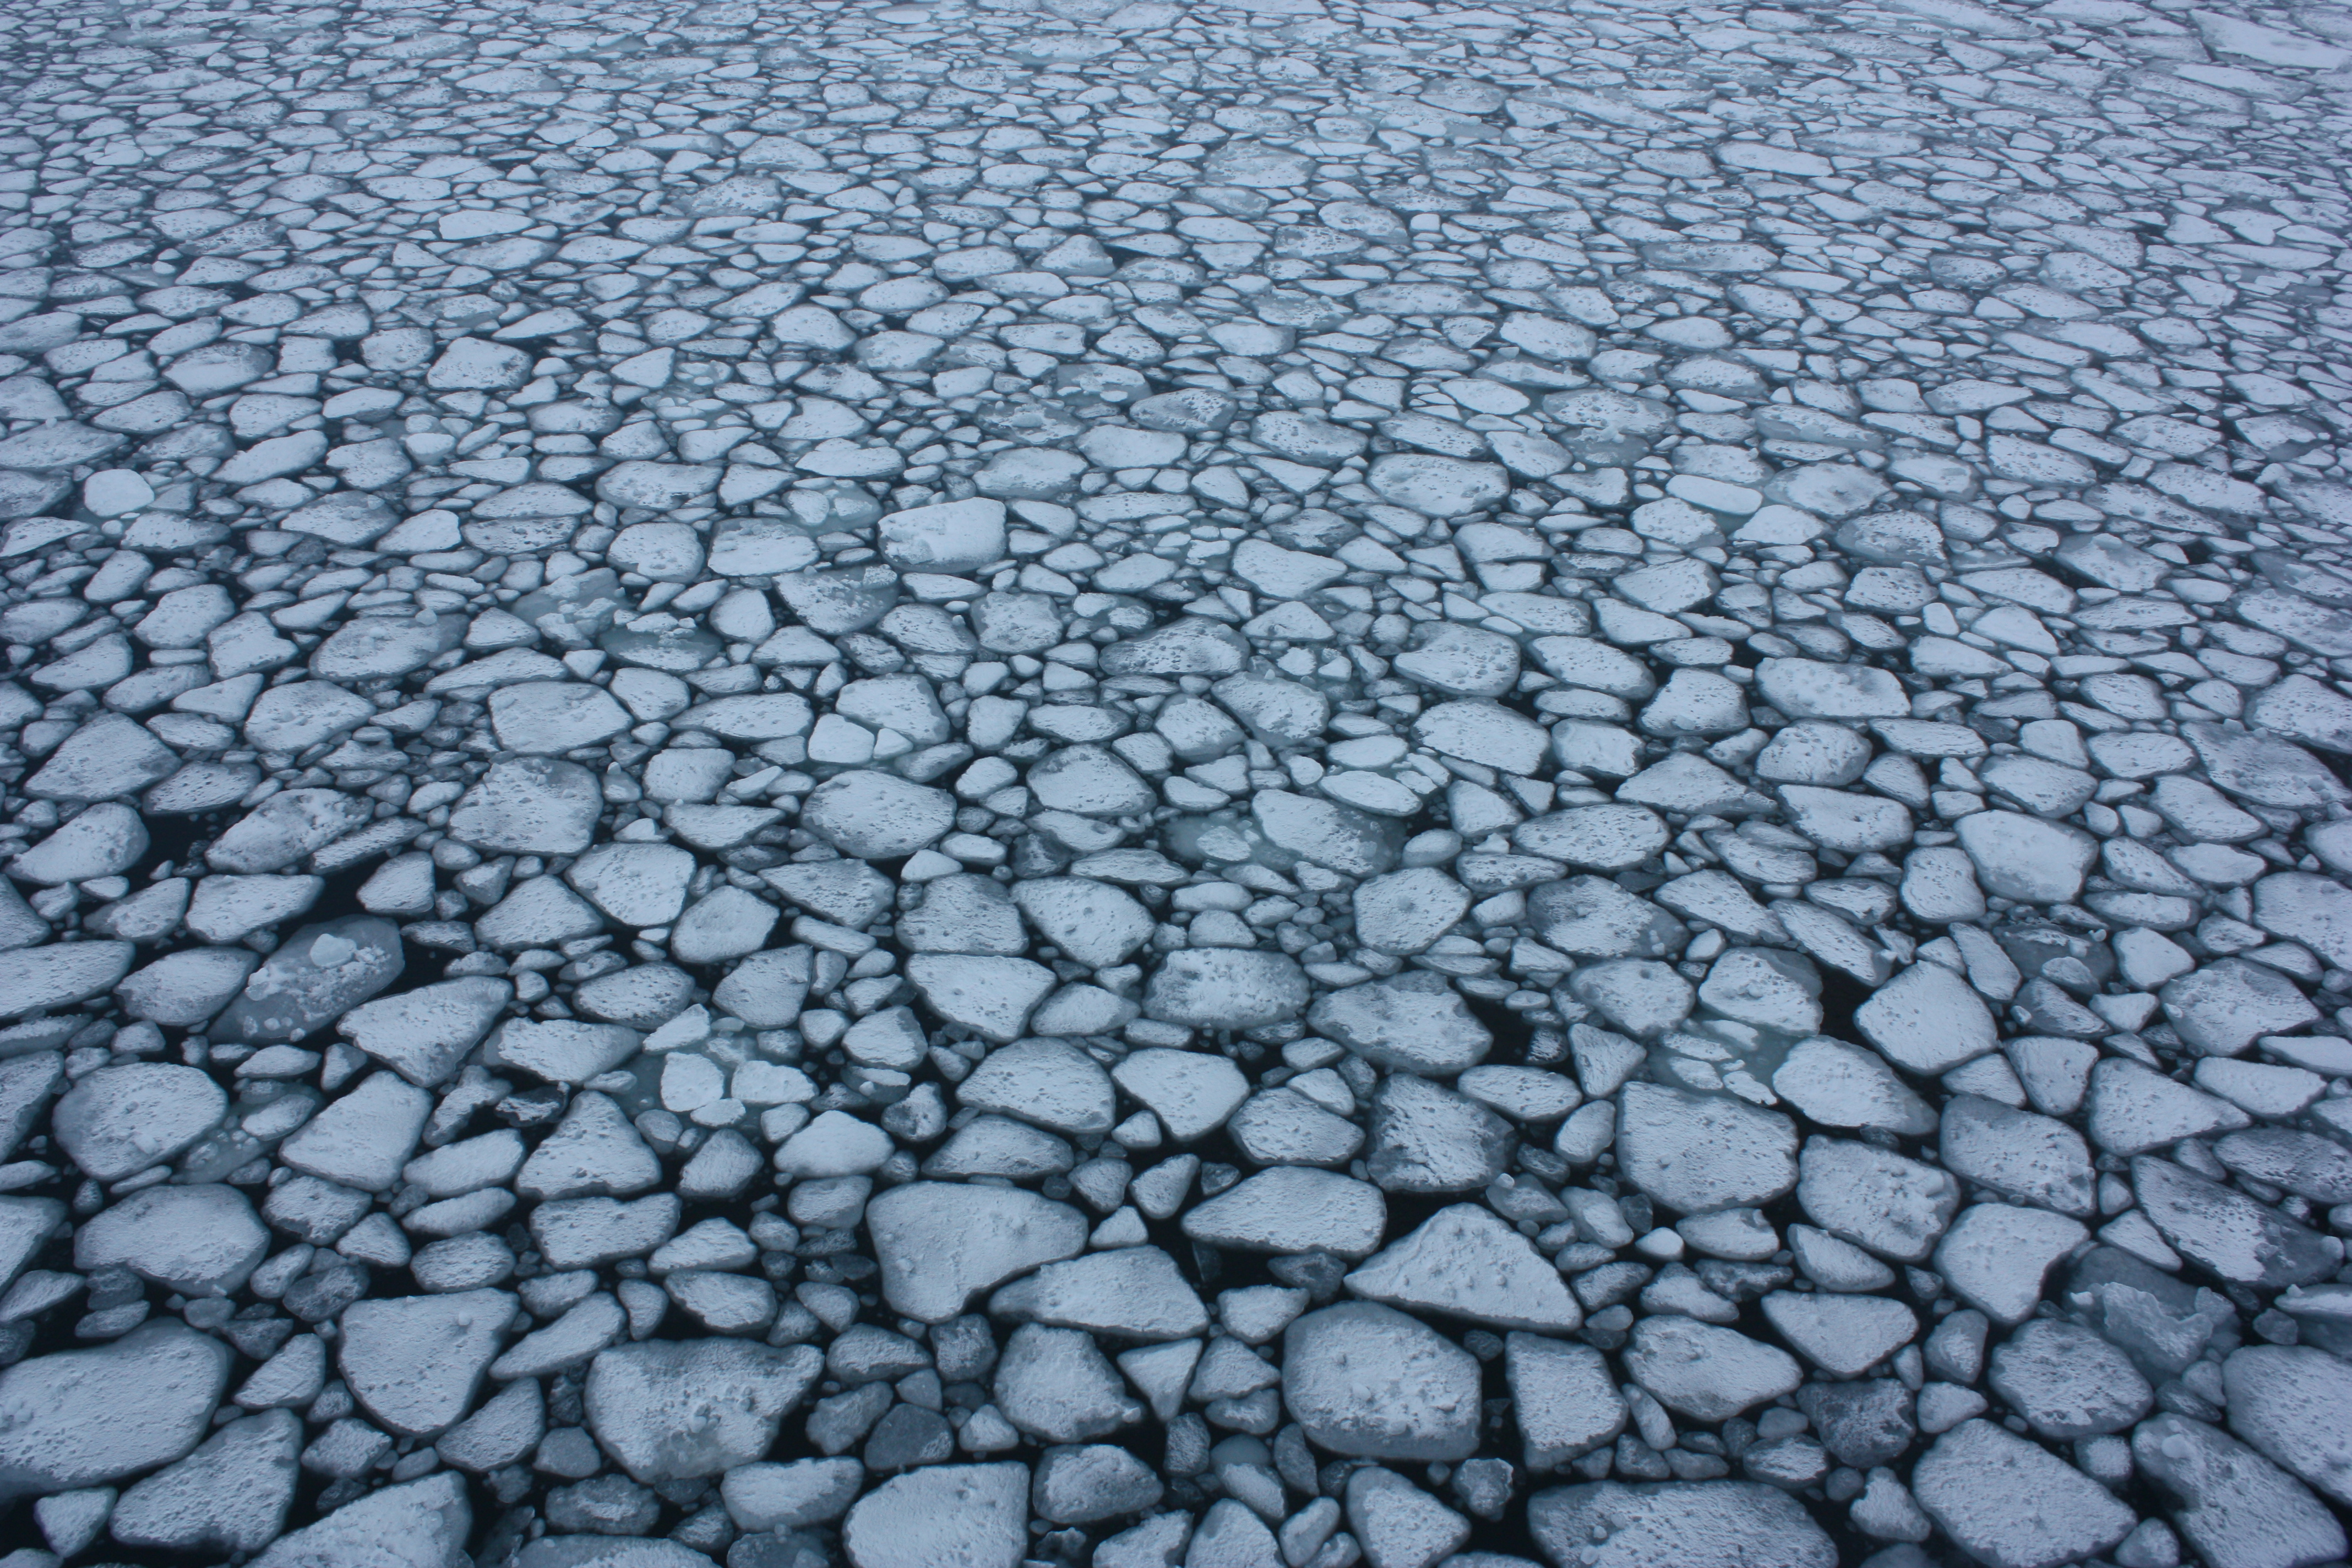
\includegraphics[width = 0.6\linewidth]{Chapter2_Theory/images/sea_ice.JPG}
    \caption{Sea ice in St. Jonsfjorden, Svalbard on 22 April at 23:00 UTC, 2018 (photograph: Private)}
    \label{fig:sea_ice}
\end{figure}


\section{Atmospheric Radiation}\label{sec:atm_rad}

The Earth's energy balance is the balance between the incoming shortwave radiation from the Sun and the \acrfull{olr} that the Earth emits to space. The average temperature on Earth is fairly constant. Thus, radiant energy from the sun that is absorbed by the earth-atmosphere system must be re-emitted in order for the equilibrium energy state to be maintained. The emitted energy from the Earth is referred to as thermal \acrfull{ir} (\cite{Liou_AtmRad}, \cite{SeinfeldSpyros}). 

\medskip

Any imbalance occurring in the the Earth-atmosphere system due to external agents is quantified as the \acrfull{rf} (\cite{IPCCchapter8}, \cite{Bowman2013}). RF is usually expressed in watts per square meter over a particular period of time, such as pre-industrial to present day (\cite{IPCCchapter8}). The estimated RF change due to tropospheric $\chem{O_3}$ since pre-industrial times is estimated to be 0.40 (0.20 to 0.60) Wm$^{-2}$ (\cite{IPCCchapter8}). This estimate is, however, somewhat uncertain partly due to the quality of observations made in the late 1800s (\cite{Tarasick2019}).


\subsection{The Radiative Properties of Ozone}\label{sec:rad_ozone}

Photodissociation of a molecule can occur when the energy of the photon exceeds the binding energy between the molecule's components (\cite{SeinfeldSpyros}). The photodissociation of ozone: $\chem{O_3} + hv \rightarrow \chem{O_2} + \chem{O}$, can yield various electronic states of the products \chem{O} and $\chem{O_2}$ depending on the wavelength of the incident radiation, with the singlet-D oxygen atom, $\chem{O}(^1\chem{D})$ being the most important electronically excited species of the atmosphere as its reaction with water vapor is a source of \chem{OH} radicals, enhancing the oxidation capacity of the atmosphere (\cite{SeinfeldSpyros}).


\medskip

The absorption spectra of ozone is varying according to the strength of the chemical bands in the molecule. The strongest band (Hartley band - $\chem{O(^3P)}$ formation) absorbs highly energetic \acrfull{uv} radiation from the sun in the upper stratosphere and mesosphere in the wavelength range 242-310 nm. The UV absorption spectrum of $\chem{O_2}$ is strongly connected to the formation of ozone, and absorbs in the range of 100-242 nm in the thermosphere, mesosphere and stratosphere. At about 50 km altitude, the maximum ozone absorption occurs in the Hartley band. In the lower stratosphere and troposphere, ozone absorbs solar flux in the range 310-400 nm (Huggins bands - $\chem{O(^3P)}$ formation). The weakest band (Chappuis bands) absorbs in the visible- and near IR region in the troposphere. The absorption range is 400-850 nm (\cite{Liou_AtmRad}). 



\medskip 

In the thermal infrared, ozone absorbs in two main bands, which are in the 9.6 and 14.27 $\mu$m regions. The latter band is overlapped by the $\chem{CO_2}$ 15 $\mu$m band. The atmospheric window is the wavelength range in which the atmosphere is relatively transparent. Thus, most IR absorption occurs outside the wavelength region 8-12 $\mu$m (\cite{AtmModFund}), which makes the 9.6 band the most important absorption band for ozone (\cite{Liou_AtmRad}, \cite{Myhre1997}). Due to it's absorption in the IR region, ozone is a gas that contributes to the greenhouse effect, i.e. it contributes to the trapping of thermal IR which leads to heating of the atmosphere (\cite{Liou_AtmRad}).

\medskip

%The column abundance of $\chem{O_3}$ is usually expressed in \acrlong{du}s. It is the measure of the thickness the column of ozone would have the whole atmosphere's content of ozone was compressed to a single layer of pure $\chem{O_3}$. One \acrshort{du} is equivalent to $2.69\times10^{16} molecules \chem{O_3} cm^{-2}$ (\cite{SeinfeldSpyros}). If the ozone concentration as a function of altitude is $n_{\chem{O_3}}(z) molecules cm^{-3}$, the $\chem{O_3}$ column burden is: 

%\begin{equation}
%    \bar{n}_{\chem{O_3}}(z) = \int_0^\infty n_{\chem{O_3}}(z)dz molecules cm^{-2}
%    \label{eqn:o3_column_burden}
%\end{equation}


%To find the relation of $\bar{n}_{\chem{O_3}}$ to DU, the thickness of the layer of pure $\chem{O_3}$ at 273 K and 1 atm needs to be determined. Over $1 cm^2$ of area, this corresponds to $\bar{n}_{\chem{O_3}}$ molecules of $\chem{O_3}$. The volume occupied by this number of molecules of $\chem{O_3}$ can be written as $V = 1 (cm^2)\times h(cm)$. One DU corresponds to a thickness, $h$, of $0.001 cm$. From the ideal gas-law:




\section{Ozone and its precursors}\label{sec:ozone_and_precursors}

Ozone is a colorless gas that impacts the life on our planet in different ways, depending on the location of it's occurrence. If situated in the stratosphere (the ozone layer) it absorbs harmful UV radiation from the Sun in the range of 100-315 nm, and is thus essentially functioning as a shield for the planet (\cite{SeinfeldSpyros}). However, if located in the lower troposphere, ozone affects human health and vegetation. Concentrations above 0.1 \acrfull{ppm} interferes with the growth of plants, and has unhealthy impacts on humans (\cite{AtmModFund}). Typical concentrations in the free troposphere range from 20 to 40 \acrfull{ppb} near sea level and from 30 to 70 ppb at higher altitudes. In moderately to severely polluted urban areas, concentrations may range from 0.01 ppm to 0.35 ppm (\cite{AtmModFund}).  

\medskip

Stratospheric ozone has a natural origin, resulting from the photolytical decomposition of $\chem{O_2}$ followed by the oxygen atom reacting with another $\chem{O_2}$ molecule, thus producing two $\chem{O_3}$ molecules. The ozone molecules themselves may continue to react with other anthropogenic and/or naturally occurring stratospheric molecules. Generally, the concentration of $\chem{O_3}$ in the stratosphere is in steady-state due to the balance of it's production and destruction. At the peak of the ozone layer, the $\chem{O_3}$ mixing ratio is about 12 ppm (\cite{SeinfeldSpyros}).  

\medskip

In the troposphere, ozone is a secondary pollutant resulting from two major classes of precursors; volatile organic compounds (VOCs) and oxides of nitrogen ($\chem{NO_x} = \chem{NO} + \chem{NO_2}$). In urban areas, $\chem{NO_x}$ mixing ratios range from 5 to 20 ppb. In rural areas, concentrations are about 1 ppb, and in remote areas, concentrations range from 10 to 100 ppt. In remote areas, ozone formation is sustained by $\chem{CH_4}$ and \chem{CO} through reactions with \chem{OH} (\cite{Cadle1970}, \cite{Levy1971}, \cite{SeinfeldSpyros}). The production of ozone is thus usually limited by the access of $\chem{NO_x}$ and $\chem{HO_x} (\chem{HO} + \chem{HO_2})$ (\cite{Levy1971}). The main removal pathways in the troposphere are through photolysis and through reaction with $\chem{HO_2}$ (\cite{SeinfeldSpyros}).

\medskip

One of the features of the stable Arctic boundary layer is the Arctic front. The front acts as a transport barrier that isolates the Arctic lower troposphere towards lower latitudes (\cite{BARRIE1986643}). In order to transport polluted air to the Arctic lower troposphere on a timescale of a few weeks, the source region of the pollution must be cold enough as well as located north of the Arctic front, which may extend down to about 40 $^o$N in January (\cite{BARRIE1986643}, \cite{AMAP2015}). 


\medskip

Both in the troposphere and the stratosphere, the $\chem{O_3}$ photolysis occurs, which produces both ground-state \chem{O} (Reaction \ref{rqn:groundstate_O2}) and excited singlet $\chem{O(^1D)}$ ((Reaction \ref{rqn:excited_O2}) oxygen atoms (\cite{SeinfeldSpyros}).

\begin{reaction}
    \chem{O_3} + hv \rightarrow \chem{O_2} + \chem{O}
    \label{rqn:groundstate_O2}
\end{reaction}

\begin{reaction}
    \chem{O_3} + hv \rightarrow \chem{O_2} + \chem{O(^1D)}
    \label{rqn:excited_O2}
\end{reaction}

The ground-state oxygen atom rapidly reacts with an oxygen molecule to re-form ozone, thus forming a null-cycle (Reaction \ref{rqn:ozone}).

\begin{reaction}
    \chem{O} + \chem{O_2} + \chem{M} \rightarrow \chem{O_3} + \chem{M}
    \label{rqn:ozone}
\end{reaction}

Reaction \ref{rqn:ozone} is the most significant source of ozone in the atmosphere (\cite{SeinfeldSpyros}). The excited oxygen atom, however must react with another atmospheric species to rid itself from excess energy. Most often, it collides with $\chem{N_2}$ or $\chem{O_2}$, which removes the excess energy, quenching it back to it's ground state (\cite{Levy1971}). Every now and then, however, the excited oxygen atom may react with $\chem{H_2O}$ to form \chem{OH} radicals (Reaction \ref{rqn:OH})(\cite{SeinfeldSpyros}). 

\begin{reaction}
    \chem{O(^1D)} + \chem{H_2O} \rightarrow 2\chem{OH}
    \label{rqn:OH}
\end{reaction}

This is the only gas-phase reaction in the troposphere that is able to break the \chem{H-O} bond in $\chem{H_2O}$ (\cite{SeinfeldSpyros}). Tropospheric ozone is thus increasing the oxidizing capacity of the troposphere as it is acting as a precursor for \chem{OH} (Reaction \ref{rqn:oh_o3}). In remote regions, ozone loss by $\chem{HO_x}$ can be an important mechanism when \chem{NO}-concentrations are low (Reaction \ref{rqn:ho2_o3})(\cite{Jacob1999}). 


\begin{reaction}
    \chem{OH} + \chem{O_3} \rightarrow \chem{HO_2} + \chem{O_2}
    \label{rqn:oh_o3}
\end{reaction}
\begin{reaction}
    \chem{HO_2} + \chem{O_3} \rightarrow \chem{OH} + 2\chem{O_3}
    \label{rqn:ho2_o3}
\end{reaction}

The hydroxyl radicals interplay in a chain of reaction that results in the removal of atmospheric \chem{CO} and $\chem{CH_4}$ (\cite{Levy1971}). Oxidation of a hydrocarbon, denoted generically as \chem{RH}, by \chem{OH} produces an inorganic peroxy radical, $\chem{RO_2}$ (\cite{Jacob1999}):

\begin{reaction}
    \chem{RH} + \chem{OH} \xrightarrow{\chem{O_2}} \chem{RO_2} + \chem{H_2O}
\end{reaction}

When \chem{NO} and $\chem{RO_2}$ are present (in polluted areas), they react to produce $\chem{NO_2}$ and organic oxy radicals \chem{RO} (\cite{Jacob1999}): 

\begin{equation}
    \chem{RO_2} + \chem{NO} \rightarrow \chem{RO} + \chem{NO_2}
\end{equation}

Ozone may then be produced photochemically (i.e. the initiating step is the absorption of a photon (\cite{Cadle1970})) by the photolysis of $\chem{NO_2}$ (Reaction \ref{rqn:no2hv}) followed by Reaction \ref{rqn:ozone} (\cite{Hesstvedt1978}).


\begin{reaction}
    \chem{NO_2} + hv \rightarrow \chem{O} + \chem{NO}
    \label{rqn:no2hv}
\end{reaction}

Tropospheric ozone production is thus sustained by emissions of $\chem{NO_x}$ and hydrocarbons \cite{Jacob1999}. 





%\subsection{Influence of Nitrogen}\label{sec:influence_of_nitrogen}


%\begin{figure}
    \centering
    \includegraphics[width=0.7\linewidth]{Chapter2_Theory/images/highNOxlowNOx.jpeg}
    \caption{Ozone in ppb (lines) simulated by a regional photochemical model as a function of emission rates of anthropogenic $\chem{NO_x}$ and hydrocarbons. The thick line separates the figure into $\chem{NO_x}$-limited (top left) and hydrocarbon limited (bottom right) regimes. Figure taken from \cite{Jacob1999} and \cite{Sillmann1990}.}
    \label{fig:highnoxlownox}
\end{figure}


%In polluted regions, there is an important balance between regions with too much $\chem{NO_x}$, which generally acts as a precursor of ozone, and areas where the $\chem{NO_x}$ concentration is low enough to sustain the production of ozone depleting reactive halogens. The high concentrations of $\chem{HNO_3}$ and $\chem{H_2SO_4}$ can in theory provide the reactive surfaces for acidity dependent autocatalytic release of reactive halogens, but the efficiency of this mechanism is degraded in the case of $\chem{NO_x}$ and hydrocarbon concentrations (\cite{Simpson2015}). High concentrations of $\chem{NO_x}$ suppresses the formation of $\chem{HO_x}$, which is in turn a key component of the halogen explosion sequence. Hydrocarbons serve as sinks for reactive halogens due to their willingness to react with these rather than with ozone, and thus terminates the halogen explosion sequence (\cite{Simpson2015}). Incidents in which halogens do get activated in polluted regions, production of nitryl halides, $\chem{XNO_2}$, is considered to be a major activation process. Observations have shown that this is mostly relevant for chlorine as the reactivity and/or solubility of $\chem{BrNO_2}$ and $\chem{INO_2}$ are likely much greater than for $\chem{ClNO_2}$ \cite{Simpson2015}. 




\section{Halogen Chemistry}\label{sec:halogen_chemistry}


The halogens are a group in the periodic table consisting of fluorine, chlorine, bromine and iodine, as well as astatine\footnote{Astatine is incredibly rare and therefore not considered to be of importance in the case of ozone depletion caused by reactive halogens}. Natural occurrence of halogens and halogen-containing compounds can be found in sea water. The reactive halogens that partake in ODEs  are thought to originate from sea salt aerosols, sea ice and snow that contains sea salt aerosols (\cite{Foster2001})(These processes are explained in detail in Section \ref{sec:het_chem}). The halide anions that may be responsible for ODEs generally occur in the following abundance in sea water (higher to lower concentrations); chloride ($\chem{Cl^-}$), bromide($\chem{Br^-}$) and iodide($\chem{I^-}$) (\cite{Simpson2015}). 

\medskip

Even though bromide is less abundant than chloride, it is most prone to participate in the depletion of ozone. The reason for this is that chlorine has a similar bond strength with hydrogen as it has with hydrocarbons (such as methane). Therefore, \chem{Cl} is prone to react with hydrocarbons rather than act to deplete ozone (Reaction \ref{R:cl_ch4}).

\begin{reaction}
    \chem{Cl} + \chem{CH_4} \rightarrow \chem{HCl} + \chem{CH_3}
    \label{R:cl_ch4}
\end{reaction}

In a field study at Alert conducted by \cite{Foster2001}, they found $\chem{Br_2}$ and \chem{BrCl} molecules in relation with \acrshort{ode}. $\chem{Cl_2}$ on the other hand, was below the detection limit throughout the measuring period, indicating that \chem{BrCl} is likely to be the chlorine compound that is active in an ODE. Bromine, on the other hand, is less reactive towards hydrocarbons and readily depletes ozone in a catalytic manner.  Fluorine creates strong bonds with hydrogen, and is thus not reactive towards ozone. Aqueous iodine is less abundant than bromine and chlorine in the ocean due to it's role as a nutrient for biological systems (\cite{FinlaysonPitts2010}, \cite{Simpson2015}). 

\medskip

Thus, the main focus in this thesis will be bromine, and to a lesser extent chlorine reactive species. The reactive halogens have short lifetimes on the order of seconds to minutes and are typically only present during the day as they are activated by photolysis:

\begin{reaction}
    \chem{BrCl} + hv \rightarrow \chem{Br} + \chem{Cl}
    \label{R:19}
\end{reaction}

\begin{reaction}
    \chem{Br_2} + hv \rightarrow 2\chem{Br}
    \label{rqn:br2_hv}
\end{reaction}

Throughout this and the following section, halogen species that partake in ozone depletion will be denoted as "\chem{X}". Reactive halogens denotes radical species such as atomic halogen species, \chem{X}, and their higher oxides, \chem{XO}. Reactions \ref{R:19} and \ref{rqn:br2_hv} will then be denoted as: 

\begin{reaction}
    \chem{X_2} + hv \rightarrow 2\chem{X} 
    \label{R:1}
\end{reaction}

The absorption spectra of dihalogens lies in the actinic (visible to near-UV) part of the spectra. Thus, photolysis may occur at longer wavelengths than that of ozone photochemistry, which requires UV photons near 300 nm (Photolysis of ozone is highly dependent on the ozone column at higher altitudes, see Section \ref{sec:rad_ozone}) (\cite{Simpson2015}).

\medskip

Halogen reservoir species are nonradicals that sequester reactive halogens. These include species such as $\chem{X_2}$, $\chem{HOX}$, $\chem{XONO_2}$ and $\chem{HX}$. The halogen reservoir species are less reactive, and hence their lifetime is longer than the reactive species (\cite{Simpson2015}). Moreover, \cite{Foster2001} found that $\chem{Br_2}$ and \chem{BrCl} were produced in high amounts at the time when polar sunrise occurred. This may point to a build-up of photolabile halogen species during the polar night. A similar theory was suggested by Simpson et.al. (\cite{Simpson2018}). They found very high \chem{BrO} concentrations in airmasses in Barrow (Utquiavik), Alaska just after polar sunrise. The airmasses were found by back-trajectory to have been exposed to photolysis of $\chem{Br_2}$ prior to arrival at the station. More information about halogen sources can be found in Section \ref{sec:halogen_sources}. 



\subsection{Bromine Explosion}\label{sec:BE}

The discovery of ODEs in the troposphere due to anomalously high concentrations of reactive halogen species, bromine in particular, was made by Barrie and coworkers at Alert in Canada in 1986-1987 (\cite{BARRIE1986643}). Ozone depletion was a well known phenomena at this point, but was until then not explained (e.g. \cite{Oltmans1981}). 

\medskip

During polar spring, the amount of ozone in the polar boundary layer may decrease from tens of ppb to less than 1 ppb due to catalytic destruction by reactive halogen species (\cite{CAO}). The reaction scheme assuming bromine is the depleting agent is to a large extent summarized in Figure \ref{fig:het_react}. 

\medskip

\begin{figure}
    \centering
    \includegraphics[width=0.7\linewidth]{Chapter2_Theory/images/ODE_Finlayson-Pitts.png}
    \caption{Typical heterogeneous reaction model. The blue shaded area illustrates the condensed phase. Figure taken from \cite{FinlaysonPitts2010}}
    \label{fig:het_react}
\end{figure}


The production of halogen radicals and subsequent ozone depletion may proceed as follows (The set of reactions is taken from \cite{CAO} and \cite{Simpson2015}): 

\medskip

Reaction \ref{R:1} produces two halogen radicals, which are highly reactive. Ozone is then destroyed by reaction with the halogen radicals (Reaction \ref{R:2}).

\begin{reaction}
    \chem{X} + \chem{O_3} \rightarrow \chem{XO} + \chem{O_2}
    \label{R:2}
\end{reaction}

The halogen oxides may proceed to deplete ozone. They partition quickly between Reactions \ref{R:3}-\ref{R:5} and either reactivate by Reaction \ref{R:1}, or become radical directly.


\begin{reaction}
    \chem{XO} + \chem{XO} \rightarrow \chem{X_2} + \chem{O_2} \label{R:3} 
\end{reaction}


\begin{reaction}
    \chem{XO} + \chem{XO} \rightarrow \chem{X} + \chem{X} + \chem{O_2} \label{R:4} 
\end{reaction}


\begin{reaction}
    \chem{XO} + \chem{XO} \rightarrow \chem{OXO} + \chem{X} \label{R:5} 
\end{reaction}

The \chem{XO}-self reaction in Reaction \ref{R:4} is often considered the rate limiting step for $\chem{O_3}$ destruction. The cycle combined of Reaction \ref{R:2} and \ref{R:4} implies that ozone loss chemistry is a quadratic function of the \chem{BrO}-concentration (\cite{Hausmann1994}). The partitioning between \chem{XO} and \chem{X} is rapid, although in the polar regions, the $[\chem{XO}]/[\chem{X}]$ ratio is generally larger than one (\cite{Schmidt}). In addition to the partitioning in Reactions \ref{R:3}-\ref{R:5}, \chem{XO} may be oxidized (Reaction \ref{R:15}) or photolysed (Reaction \ref{R:20}).

\begin{reaction}
    \chem{OH} + \chem{XO} \rightarrow \chem{X} + \chem{HO_2}
    \label{R:15}
\end{reaction}

\begin{reaction}
    \chem{XO} + hv \rightarrow \chem{X} + \chem{O}
    \label{R:20}
\end{reaction}

The halogen oxides quickly photodissociate (on the order of seconds and minutes time scale) and Reactions \ref{R:2} and \ref{R:20} creates a null cycle that doesn't destroy nor produce ozone. This has an effect on the partitioning of \chem{X} and \chem{XO} species. The oxides dominate the radical form, which extends the lifetime of the $\chem{XO_x} = \chem{X} + \chem{XO}$-family as the oxides are generally less reactive than the atomic form (\cite{Simpson2015}). 


\medskip

Termination reactions that renders the \chem{XO} and \chem{X}-radicals into the reservoir species \chem{HBr} and \chem{HOBr} may proceed as follows: 


\begin{reaction}
    \chem{XO} + \chem{HO_2} \rightarrow \chem{HOX} + \chem{O_2}
    \label{R:6} 
\end{reaction}

\begin{reaction}
    \chem{X} + \chem{HO_2} \rightarrow \chem{HX} + \chem{O_2}
    \label{R:17}
\end{reaction}


\begin{reaction}
    \chem{OH} + \chem{XO} \rightarrow \chem{HX} + \chem{O_2}
    \label{R:16}
\end{reaction}


According to the box-model experiments by \cite{CAO}, the dominant halogen species after an ODE is \chem{HX}. The efficiency of ozone destruction is not only dependent on the availability of reactive bromine, but also the efficiency of reconverting reservoir species (\chem{HBr} and \chem{HOBr}) back into reactive \chem{Br}. \chem{HOBr} photolyses readily to form \chem{Br} and \chem{OH} (Reaction \ref{R:18}) (\cite{Hausmann1994}).

\begin{reaction}
    \chem{HOBr} + hv \rightarrow \chem{Br} + \chem{OH}
    \label{R:18}
\end{reaction}


The bromine explosion events involves reaction \ref{R:1}, \ref{R:2} and \ref{R:6}, with $\chem{X} = \chem{Br}$, in an autocatalytic manner by the means of heterogeneous reactions over snow- or ice surfaces (Reaction \ref{R:7}) and over aerosol surfaces (Reaction \ref{R:8}). 

\begin{reaction}
    \chem{HOBr} + \chem{X^-_{aq}} + \chem{H^+_{aq}} \xrightarrow{snow/ice} \chem{BrX} + \chem{H_2O} \label{R:7} 
\end{reaction}
\begin{reaction}
    \chem{HOBr} + \chem{HX_{aq}} \xrightarrow{aerosol} \chem{BrX} + \chem{H_2O} \label{R:8}
\end{reaction}


In which the multiphase Reactions \ref{R:7} and \ref{R:8} outlines the release of bromine radicals from the condensed phase on snow/ice surfaces or aerosol surfaces, respectively. In this case, \chem{X} may denote \chem{Br} or \chem{Cl}, normally. The full multiphase reaction is dependent on temperature, sunlight and an acidic reaction surface (\cite{Toyota}). The bromine explosion can be summed up as follows: 

\begin{align*}
    \chem{HOBr} + \chem{X^-_{aq}} + \chem{H^+_{aq}} &\xrightarrow{snow/ice} \chem{BrX} + \chem{H_2O} \\
    \chem{Br_2} + hv &\rightarrow 2\chem{Br} \\
    \chem{Br} + \chem{O_3} &\rightarrow \chem{BrO} + \chem{O_2} \\
    \chem{BrO} + \chem{HO_2} &\rightarrow \chem{HOBr} + \chem{O_2} \\
    \text{NET:} \quad \chem{X^-_{aq}} + \chem{H^+_{aq}} + \chem{HO_2} + \chem{O_3}  &\rightarrow \chem{Br} + \chem{H_2O} + 2\chem{O_2} 
\end{align*}

\medskip

The ODEs terminate when there's no ozone left to deplete, as that prohibits Reaction \ref{rqn:oh_o3}-\ref{rqn:ho2_o3} such that there will be far less $\chem{HO_x}$-species. This affects Reaction \ref{R:6}, $\chem{BrO} + \chem{HO_2} \rightarrow \chem{HOBr} + \chem{O_2}$, which again terminates the autocatalytic heterogeneous reactions that produces reactive halogen species. 

\subsubsection{Reactive Surfaces}

The reactive surface may be supplied by different media, and this is an object of many research articles (e.g. \cite{KerriAPratt2013}, \cite{Rankin}). Whichever is more significant, there is most likely a cooperation of the reactive surfaces that accelerates the bromine explosion events. The reactive surfaces are (generally): 

\begin{itemize}
    \item Newly formed sea ice: Has a higher salinity and a higher bromine content than old sea ice and sea water \cite{Rankin}
    \item Snow surfaces, with low pH
    \item Aerosol surfaces, with low pH
\end{itemize}

\subsubsection{ODEs and Halogen-Driven $\chem{NO_x}$-Loss}

Halogen driven tropospheric ozone loss globally was found by \cite{Schmidt} to be due to a combination of depletion by catalytic BE-events and a decrease in $\chem{NO_x}$-driven ozone production. This is due to halogen-driven $\chem{NO_x}$-loss which is largest in low $\chem{NO_x}$-areas, such as the polar regions. The halogen-driven $\chem{NO_x}$-loss occurs due to hydrolysis of the halogen nitrates (\cite{Schmidt}):

\begin{reaction}
    \chem{BrO} + \chem{NO} \rightarrow \chem{NO_2} + \chem{Br}
    \label{R:14}
\end{reaction}


\begin{reaction}
    \chem{BrO} + \chem{NO_2} + M \rightarrow \chem{BrONO_2} + M
    \label{R:9}
\end{reaction}


\begin{reaction}
    \chem{BrONO_2} + \chem{H_2O} \xrightarrow{aerosol} \chem{HOBr} + \chem{HNO_3}
    \label{R:13}
\end{reaction}




\subsubsection{Chlorine Reservoir Species}

In the stratosphere, $\chem{NO_2}$ and $\chem{CH_4}$ are responsible for shifting reactive chlorine species into reservoir species (\cite{SeinfeldSpyros}). \cite{Wang_2019} found that these reactions are also of relevance in the troposphere, among other reactions. Methane acts via Reaction \ref{R:cl_ch4} to form $\chem{CH_3}$. Reservoir compounds may form by the reaction of \chem{XO} and $\chem{NO_2}$: 

\begin{reaction}
    \chem{ClO} + \chem{NO_2} + M \rightarrow \chem{ClONO_2} + M
    \label{R:clono2}
\end{reaction}

\subsection{Halogen Sources}\label{sec:halogen_sources}

Sources of reactive halogens in the troposphere include photochemical degradation and oxidation of organobromines ($\chem{CHBr_3}$, $\chem{CH_2Br_2}$, $\chem{CH_3Br}$), release of bromide ($\chem{Br^-}$) and chloride ($\chem{Cl^-}$) from \acrfull{ssa} and transport from the stratosphere (\cite{Schmidt}). 

\medskip

Model studies have shown that the release of reactive halogen species from SSA is particularly relevant in polar regions (\cite{Schmidt}). While SSA is a known and certain source of reactive bromine species in the Arctic, the surface on which sea salt is transformed into gas-phase reactive halogens is somewhat unclear (\cite{Simpson2005}). SSA is formed though the breaking of waves at the ocean surface (\cite{Simpson2015}). 

\medskip

Formation of reactive halogen species though frost flowers has been suggested as a potential source. Frost flowers are ice crystals that forms on new sea ice when air that is supersaturated with water vapor condenses at the surface of the ice (\cite{GRANFORS2013124}, \cite{Kaleschke}). However, the sporadic nature and short lifetime of frost flowers points to other sources that may be more prominent as ODEs occur frequently during the polar spring. Snowpack measurements over coastal- and central Arctic \acrfull{fyi} and remote \acrfull{myi} performed by \cite{Peterson2019} revealed mostly snowpacks enriched in bromide species as a potential source of reactive bromine. This suggests that both MYI and FYI plays a role in the activation of halogens that subsequently may deplete ozone. The halides are incorporated in the snowpack by transported snow containing SSA (\cite{Toyota}, \cite{Peterson2019}). Trace bromine gases, such as \chem{HBr}, \chem{HOBr} and $\chem{BrONO_2}$, may be produced in the snowpack or deposited through mulitphase-reactions (\cite{Simpson2005}). 


\medskip


Globally, chlorine is the most abundant halide in the marine boundary layer. \chem{Cl} is released from SSA as $\chem{HCl}$ by acid displacement and photochemically as reactive halogens or their precursors. There is a difference between the halide content in the marine boundary layer in polar regions and outside polar regions. In the polar \acrshort{bl} $\chem{BrO}$ is routinely observed, whereas outside polar regions \chem{BrO} concentrations rarely exceed detection limits (\cite{Simpson2015}). 

\medskip

The ocean also provides a large source of bromine- and iodide containing halocarbons that, when emitted into the troposphere, comprise very short-lived species (VSLS) that influence ozone destruction both in the troposphere and stratosphere (\cite{ziska}, \cite{Simpson2015}). The most abundant short-lived halocarbon (containing bromine) in the atmosphere and ocean are bromoform ($\chem{CHBr_3}$) and dibromomethane ($\chem{CH_2Br_2}$). Bromoform and dibromomethane are produced by marine organisms such as macroalgae and phytoplankton (\cite{Quack2003}).


\medskip

$\chem{CHBr_3}$ and $\chem{CH_2Br_2}$ become sources of reactive bromine in the troposphere through oxidation or through photolysis of $\chem{CHBr_3}$ (\cite{Hossaini2016_chlorine}):


\begin{reaction}
    \chem{CHBr_3} + \chem{OH} \rightarrow 3\chem{Br} + \chem{Products}
    \label{R:10}
\end{reaction} 
\begin{reaction}
    \chem{CH_2Br_2} + \chem{OH} \rightarrow 2\chem{Br} + \chem{Products}
    \label{R:11}
\end{reaction}
\begin{reaction}
    \chem{CHBr_3} + hv \rightarrow 3\chem{Br} + \chem{Products}
    \label{R:12}
\end{reaction}

As $\chem{CH_2Br_2}$ is less willingly photolysed, the lifetime of this compound in the troposphere is slightly longer ($94 (84-114)$ days) than $\chem{CHBr_3}$ ($15 (13-7)$ days) (\cite{Hossaini2016_chlorine}).

\medskip

Reactive bromine species and their precursors may also be transported, either within the Arctic boundary layer (\cite{Luo2018}, \cite{Schmidt}), or from the stratosphere (\cite{Hossaini2016_chlorine} and references therein). 


\cleardoublepage

\setcounter{chapter}{2} 
\chapter{Theoretical background: Processes Implemented in the CTM3}\label{Chap:CTM3theory_ocean_hetReact}

Some of the processes that are implemented in the Oslo CTM3 requires some further explanation. Here, I will cover the theory behind the implementation of emissions of organic halogen species and the heterogeneous reaction surfaces.

\section{Oceanic emissions of halocarbons}\label{sec:oceanic_emissions}


The ocean is a natural source of gaseous halocarbons, and is therefore used here as a source needed for the bromine explosion to occur. Methyl halides ($\chem{CH_3X}$) and polyhagenated species ($\chem{CHBr_3}$, $\chem{CH_2Br_2}$) are released from the ocean, but methyl halides (particularly $\chem{CH_3Br}$) may also be emitted by biomass burning (\cite{SeinfeldSpyros}). 

\medskip

Bromoform ($\chem{CHBr_3}$) and dibromomethane ($\chem{CH_2Br_2}$) are used as the oceanic sources of bromine in this implementation. The anthropogenic signal of methyl halides are not taken into consideration in this thesis. Nor are the difference in lifetime ($\chem{CH_3Br} \sim$ 1 month, $\chem{CH_2Br_2} \sim$ 4 months) as well as seasonal variations. 


\medskip

Bromoform, $\chem{CH_3Br}$, is added as a source from the ocean based on the emission scenario suggested by \cite{Liang2010} (scenario A, Figure \ref{fig:Liang2010}). This scenario was chosen as it has latitudinal-dependent emission field covering the whole globe. The global emissions estimated by \cite{Liang2010}, scenario A, were 425 Ggyr$^{-1}$ of $\chem{CHBr_3}$ and 57 Ggyr$^{-1}$ of $\chem{CH_2Br_2}$, respectively.

\medskip

The thought behind the implementation (the variable \texttt{POLL\_CHBr3}) is that it contains the emissions from both $\chem{CHBr_3}$ and $\chem{CH_2Br_2}$. The reason for this is that there was already an organic halogen existing in the CTM3, methyl bromide ($\chem{CH_3Br}$), which would only be used by the model when the stratosphere was activated (which was not the case in my runs). Thus, this was used for the mapping of the concentration of $\chem{CHBr_3}$ and $\chem{CH_2Br_2}$ instead. To simplify this source further, $\chem{CH_2Br_2}$ was added to the emission scheme in Figure \ref{fig:Liang2010} by a scaling factor based on the global emissions. 

\medskip

The scaling factor was calculated by finding the yield of bromine from both $\chem{CHBr_3}$ and $\chem{CH_2Br_2}$ based on reactions \ref{R:10} and \ref{R:11}, and expressing this in terms of $\chem{CHBr_3}$. 

\begin{align*}
    \chem{X} & = 57 Gg \chem{CH_2Br_2}yr^{-1} \\
    \chem{Y} & = 425 Gg \chem{CHBr_3}yr^{-1} 
\end{align*}

The bromine yield, \chem{Z}, from Reactions \ref{R:10} and \ref{R:11} is then: 

\begin{align*}
    \chem{Z} & = \Big(3\cdot\Big(\frac{X}{M_{\chem{CH_2Br_2}}}\Big) + 2\cdot\Big(\frac{Y}{M_\chem{CHBr_3}}\Big)\Big)\cdot M_{\chem{Br}} \\
    & = \Big(3\cdot\Big(\frac{425 Gg \chem{CHBr_3}yr^{-1}}{252.73 g mol^{-1}}\Big) + 2\cdot\Big(\frac{57 Gg \chem{CH_2Br_2}yr^{-1}}{173.83 g mol^{-1}}\Big)\Big)\cdot79.90 g mol^{-1} \\
    & = 455 Gg\chem{Br}yr^{-1}
\end{align*}

The emission of $\chem{CHBr_3}$, had this been the only source of bromine, is expressed by $Y'$, which is: 

\begin{align*}
    \chem{Y'} & = \frac{1}{3}\cdot\frac{252.73 g mol^{-1}}{79.90 g mol^{-1}}\cdot455.49Gg\chem{Br}yr^{-1} \\
    & = 479.73 Gg \chem{CHBr_3}yr^{-1}
\end{align*}

This is used in the scaling factor, $f$:

\begin{equation*}
    f = \frac{\chem{Y'}}{Y} \approx 1.13
\end{equation*}


Emissions are then found according to their latitudinal band, and whether the grid box is located over ocean or the coast (for more information about the actual implementation, see Section \ref{sec:tropchem_oslo}). If the location is above 50 $^o$ North over ocean, for example, the emission is taken to be $0.05\times10^{-13}$ kgm$^{-2}$s$^{-1}\times k$. (The conversion to molecules cm$^{-3}$s$^{-1}$ can be seen in Section \ref{sec:tropchem_oslo}). 


\subsection{Emission inventory}

The emission inventory of $\chem{CHBr_3}$ and $\chem{CH_2Br_2}$ by \cite{Liang2010} was compared against observations and other emission inventories by \cite{Hossaini2013}. The results can be seen in Figures \ref{fig:Hosaini_fig5} and \ref{fig:Hosaini_fig6} in the Appendix. They show a reasonable agreement between the observations and mixing ratios suggested by \cite{Liang2010} for the stations \acrfull{alt}, \acrfull{brw} and Summit (SUM), which are of most relevance in this setting. The inventory, however is rather crude and simple as it does not take into account seasonality, extrapolar results of agreement with observations. 


\begin{figure}
    \centering
    \includegraphics[width = 0.5\textwidth]{Chapter3_Theory_ocean_hetReact/images/liang_etal_2010.png}
    \caption{Global emission distribution of $\chem{CHBr_3}$. Scenario A is applied for the \chem{CHBr_3} with emissions taken as the half point of the colorbar. Image taken from \cite{Liang2010}}
    \label{fig:Liang2010}
\end{figure}



\section{Heterogeneous chemistry}\label{sec:het_chem}

Bimolecular reactions are reactions in which two chemical species react and produce a different set of species (\cite{Jacob1999}). The reaction can be written as: 

\begin{equation*}
    A + B \rightarrow C + D
\end{equation*}

The reaction rate, $k$, is the time rate of change of a concentration of the reactant in the reaction (\cite{AtmModFund}). It is given by: 

\begin{equation*}
    -\frac{d}{dt}[A] = -\frac{d}{dt}[B] = \frac{d}{dt}[C] = \frac{d}{dt}[D] = k[A][B]
\end{equation*}

in which the bracketed species $[]$ denotes the number densities (in this case the number of molecules per $cm^3$) and $k$ is the second-order deposition-rate constant for the reaction in $cm^3\text{molecule}^{-1}s^{-1}$. The product $[A][B]$ is proportional to the frequency of collisions. A bimolecular reaction could also be a self-reaction, in which $B = A$ and the reaction rate would be:

\begin{equation*}
    -\frac{d}{dt}[A] = -\frac{d}{dt}[A] = \frac{d}{dt}[C] = \frac{d}{dt}[D] = k[A]^2
\end{equation*}

\subsection{Heterogeneous reactions on aerosol surfaces (Reactions \ref{R:8} and \ref{R:13})}\label{sec:aerosol_react}

The implementation of the aerosol Reactions \ref{R:8} and \ref{R:9} is based on the method described by \cite{CAO} and \cite{schwartz1986}. An overview of the constants used can be found in Table \ref{tab:constants}.

\medskip

The production rate of $\chem{Br_2}$ molecules for Reaction \ref{R:8} is given as: 

\begin{equation*}
    \frac{d}{dt}[\chem{Br_2}] = -\frac{d}{dt}[\chem{HOBr}] = k[\chem{HOBr}]
\end{equation*}

which has the first-order reaction-rate constant: 

\begin{equation*}
    k = \big(\frac{a}{D_g} + \frac{4}{v_{therm}\gamma}\big)^{-1}\alpha_{eff}
    \label{eq:reaction_rate_const}
\end{equation*}

in which $a$ is the aerosol radius, $D_g$ is the molecular diffusivity in the gas-phase, and the ratio $a/D_g$ represents the molecular diffusion limit. Following \cite{CAO}, the values of these are $a = 0.45 \mu m$ and $D_g = 0.2 cm^2s^{-1}$. 

\medskip

$v_{therm}$ in Equation \ref{eq:reaction_rate_const} is the mean molecular speed of \chem{HOBr} given as $v_{them} = \sqrt{8RT/(\pi \chem{M_{HOBr}})}$ in which $R$ is the universal gas constant (units $[Latm/Kmol]$), $T$ is the absolute temperature (units $[K]$) and $\chem{M_{HOBr}}$ is the molas mass of \chem{HOBr} (units $[g/mol]$). 

\medskip

$\gamma$ is the uptake coefficient or reaction efficiency of \chem{HOBr} on sea salt aerosols, i.e. the probability that the reaction will occur (\cite{SeinfeldSpyros}).

\medskip

$\alpha_{eff}$ is the surface-volume coefficient, i.e. the ratio of the total aerosol surface area, $A_{\text{aerosol}}$, and the total volume, $V$ (units $[cm^2cm^{-3}]$).
 
\medskip

The production rate of $\chem{Br_2}$ in Reaction \ref{R:8} is limited by the absorption of \chem{HOBr} and \chem{HBr}/\chem{HCl} in the suspended aerosol particles (\cite{CAO}). \cite{Hanson1994} expressed the effective uptake coefficient on small drops as: 

\begin{equation}
    \frac{1}{\gamma} = \frac{1}{\alpha}+ \frac{v_{therm}}{4H^*RT\sqrt{k_{liq}^ID_{liq}}f(q)}
    \label{eq:upt_coeff}
\end{equation}

\medskip

$R$ is the universal gas constant, $T$ is the temperature.

\medskip

$D_{liq}$ is the liquid phase diffusion coefficient (proportionality factor implying that a mass of the substance diffuses through a unit surface in a unit time at a concentration gradient of unity). 

\medskip

in which $\alpha$ is the mass accommodation coefficient. This quantity describes the probability that a gas or vapour particle will stick upon collision with the surface of a particle, where $0\leq\alpha\leq1$ (\cite{SeinfeldSpyros}). Following \cite{CAO}, this will be taken as unity. 

\medskip

$H^*$ is the effective Henry's law constant for the species in question. The Henry's law coefficient, $H$, is a proportionality factor between the amount of dissolved gas and it's partial pressure in the gas phase (\cite{Sander2015}, see also Section \ref{sec:wet_dep_henrys_law}).  

$k_{liq}^I$ is the first-order liquid reaction rate constant for the species in question, calculated by: 

\begin{equation}
    k_{liq}^I = k_{liq}^{II}[\chem{X}]_{liq}= k_{liq}^{II}H^*_\chem{X}P_\chem{X}
\end{equation}

In which $H^*_\chem{X}$ is the effective Henry's law constant for the species and $P_\chem{X}$ is it's partial pressure.

\medskip

$f(q)$ is determined by: 

\begin{equation}
    f(q) = \coth{q} -\frac{1}{q} = \frac{1}{\tanh{q}} -\frac{1}{q}
\end{equation}

where $q = a\sqrt{\frac{k_{liq}^I}{D_{liq}}}$, is a dimensionless quantity called the diffuso-reactive parameter. This is used to calculate the uptake rates (\cite{Hanson1994}). 


\subsubsection{Heterogeneous reactions over snow and ice surfaces (Reactions \ref{R:7})}\label{sec:snow_ice_react}


The implementation of the heterogeneous reactions over snow/ice surfaces also follows the method by \cite{CAO}. 

\medskip

The change in concentration for Reactions \ref{R:7} can be given as: 

\begin{equation*}
    -\frac{d}{dt}[\chem{HOBr}] = k[\chem{HOBr}]
\end{equation*}

in which the deposition-rate constant, $k$, is: 

\begin{equation*}
    k = \frac{v_d}{L_{mix}}\beta
\end{equation*}

Thus, the deposition-rate constant depends on the deposition velocity, $v_d$, at the snow/ice surface, the height of the boundary layer, $L_{mix}$ and the reactive surface ratio coefficient, $\beta$. 

\medskip

The deposition velocity, $v_d = (r_a + r_b + r_c)^{-1}$, is dependent on three resistances which are: 

\begin{itemize}
    \item The aerodynamic resistance, $r_a$. This is the resistance of the turbulent transport to bring the gas from the atmosphere to the surface, approximated as: $1/(u\kappa^2)(\ln(z/z_0))^2$, where $u = 8 ms^{-1}$ is the wind speed, $\kappa = 0.4$ is the Von Karman constant, $z$ is the surface layer height, approximated as the lower $10\%$ of the boundary layer, i.e. $z = 0.1L_{mix}$, and $z_0$ is the surface roughness length which is approximated as $10^{-5} m$ for ice surfaces. $r_a$ is therefor dependent on local properties. 
    \item The quasi-laminar layer resistance, $r_b$, is the ability of molecular diffusion to transfer gas across a liquid-laminar layer above the surface. It is thus given as $r_b = z_0/D_g$
    \item The resistance due to the reaction loss, $r_c$ is given as $r_c = 4/v_{therm}\gamma$. The uptake coefficient is taken as $\gamma = 0.06$ including the assumption that the source of $\chem{H^+}$ and halogen ions are limitless at the snow/ice surface. 
\end{itemize}

$L_{mix}$ denotes the typical stable boundary layer height which may, in Polar regions, range from near-zero up to approximately 1000 m depending on. Consequently, the deposition velocities vary.

\medskip

$\beta$ is the ratio of the total reactive surface (induced by the structure of snow/ice surfaces) to a flat area. Thus, for a completely flat surface, $\beta$ equals 1. 

\begin{table}[ht]
\centering
\resizebox{\columnwidth}{!}{%
\begin{tabular}{|llll|}
\hline
\textbf{Variable} & \textbf{Quantity}    & \textbf{Unit}       & \textbf{Description}                                       \\ \hline
\multicolumn{4}{|c|}{\textbf{\chem{HOBr}}}                                                                 \\ \hline
$\alpha$          & $1.0$                & Dimensionless       & Mass accommodation coefficient                             \\
$\alpha_{eff}$    & $1.0 \times 10^{-6}$ & $cm^{-1}$           & Surface-volume coefficient                                 \\
$a$               & $0.45$               & $\mu m$             & Typical aerosol radius                                     \\
$\beta$           &                      & Dimensionless       & Ratio of the total reactive surface area to a flat surface \\
$D_{liq}$         & $5.0\times10^{-6}$   & $cm^2s^{-1}$        & Liquid phase diffusion coefficient                         \\
$D_g$             & $0.2$                & $cm^2s^{-1}$        & Molecular diffusivity                                      \\
$H^*$             & $1.7 \times10^4$     & $molL^{-1}atm^{-1}$ & Effective Henry's law constant                             \\
$M_{\chem{HOBr}}$ & $96.91\times10^{-3}$ & $kg mol^{-1}$       & Molar mass of \chem{HOBr}                 \\ \hline
\multicolumn{4}{|c|}{\textbf{\chem{HBr}}}                                                                  \\ \hline
$H^*$             & $3.0\times10^{8}$    & $molL^{-1}atm^{-1}$ & Effective Henry's law constant                             \\
$k_{liq}^{II}$    & $5.0\times10^{4}$    & $L mol^{-1}s^{-1}$  & Second order liquid rate reaction constant                 \\ \hline
\multicolumn{4}{|c|}{\textbf{\chem{HCl}}}                                                                  \\ \hline
$H^*$             & $3.0\times10^{6}$    & $molL^{-1}atm^{-1}$ & Effective Henry's law constant                             \\
$k_{liq}^{II}$    & $1.0\times10^{5}$    & $L mol^{-1}s^{-1}$  & Second order liquid rate reaction constant                 \\ \hline
\multicolumn{4}{|c|}{\textbf{$\chem{BrONO_2}$}}                                                                             \\ \hline
$\gamma$          & $0.06$               & Dimensionless       & Effective uptake coefficient                               \\ \hline
\end{tabular}
}
\caption{Overview of constants taken from \cite{CAO}}
\label{tab:constants}
\end{table}



\subsection{Photochemistry}

For photochemical reactions, the rate expression is (\cite{AtmModFund}):

\begin{equation*}
    A + hv \rightarrow B + C
\end{equation*}

and the rate expression is: 

\begin{equation*}
    \frac{d[A]}{dt} = -J[A]
\end{equation*}

In which $J$ is a first-order photolysis rate coefficient of species $A$ (units: $s^-1$). 

\section{Wet deposition and Henry's law}\label{sec:wet_dep_henrys_law}

Henry's law expresses the proportional relationship between the amount of gaseous and dissolved gas (\chem{A}) in equilibrium (\cite{SeinfeldSpyros}): 

\begin{equation*}
    \chem{A(g)} \rightleftharpoons \chem{A(aq)}
\end{equation*}

The proportionality factor is dependent on the partial pressure of \chem{A} in the gas phase and the dissolved \chem{A} such that: 

\begin{equation}
    [\chem{A(aq)}] = H_Ap_A
    \label{eq:Henryslaw}
\end{equation}

In which $H_A$ is the Henry's law coefficient and $p_A$ is the partial pressure of \chem{A(g)}. 

\medskip

In this context, and widely used by atmospheric chemists, the Henry solubility, $H^{cp}$ is applied (\cite{Sander2015}). Rearranging Equation \ref{eq:Henryslaw} gives: 

\begin{equation}
    H^{cp} \equiv \frac{C_A}{p_A}
    \label{eq:HenrySol}
\end{equation}

The temperature dependence of the Henry's law coefficient, which is an equilibrium constant, can be described by the van't Hoff equation (\cite{Sander2015} and references therein): 

\begin{equation*}
    \frac{d\ln(H)}{d(1/T)} = \frac{-\Delta_{sol}H}{R}
    \label{eq:vantHoff}
\end{equation*}

In which $\Delta_{sol}H$ is the change in enthalpy of dissolution ($H$ in this case does not refer to the Henry's law constant). $R$ is the universal gas constant. 


Hva er wet deposition? Hvordan relateres Henrys law til wet deposition?


The Henry's law constants can be seen in Section \ref{sec:scav_wet} in Table \ref{tab:Henrys_law}. 


\section{3-body reactions}


Reactions \ref{R:clono2} and \ref{R:13} were implemented by using the 3 body reaction scheme for their reaction rate constants. \cite{SovdeManual}. 

Smooth og grei!
\cleardoublepage

\setcounter{chapter}{3}
\chapter{Theoretical Background: Oslo CTM3}\label{chapt:OsloCTM3}

This chapter covers some of the functionality of the Oslo CTM3 that is of importance in the implementation of the halogen chemistry (Theory outlined in Chapter \ref{Chap:CTM3theory_ocean_hetReact} and the implementation process outlined in Chapter \ref{chap:CTM3_Setup}).

\section{The Oslo CTM3}

The Oslo CTM3 is a three-dimensional global chemical transport model. The model was developed at the Department of Geosciences at the University of Oslo and later at \acrfull{cicero} (\cite{SovdeManual}). It operates offline driven by historical weather data from the \acrfull{ecmwf} \acrfull{openifs} model. The meteorological data is updated (offline) and stored every 3rd hour. The model spin-up time is 12h starting from an analysis at noon the day before (\cite{Sovde2012}). 

\medskip

The tropospheric chemistry in the CTM3 is a stand-alone module, while the stratosphere module requires the troposphere. Thus, there is a possibility of turning off the stratosphere to better isolate chemical processes occurring in the troposphere. In that case, the tropospheric species that are advected throughout the stratosphere are allowed to do so, but are not affected by any real chemistry. The species that are photolyzed in the stratosphere are instead set to decay at fixed rates, and species that have stratospheric origin (such as ozone and $\chem{NO_x}$) are set to model climatological values (climatological values produced by the CTM3 with stratosphere) (\cite{Sovde2012}).

\section{Transport of Species}\label{sec:CTM3_transport}

The transport time step in the Oslo CTM3 is usually 15 minutes for boundary layer mixing. For species with a much shorter lifetime with this, the concentration may change during the time step. The transport scheme in the CTM3 is therefore divided into transported- and non-transported species (\cite{SovdeManual}).

\medskip

The advection scheme in Oslo CTM3 is the UCI CTM transport core documented by \cite{Prather2008}. This is a 3D isotropic (same second order moment in all directions) advection scheme, where the zonal (U) and meridional (V) metereological fields are used to calculate the vertical field (W). An important feature of the advection scheme is the handling of the transport at the poles. Each polar-"pie" box is combined with it's adjacent lower-latitude box (which conserves all moments) before [U] and [V] transport and restored to individual boxes afterwards, assuming unchanged polar pie air mass (\cite{Sovde2012}). 


\section{Photochemistry}\label{sec:CTM3_photochemistry}

The photodissocation rates (J-values) in $[s^{-1}]$ are calculated online using the fast-JX method, version 6.7c (\cite{FastJX}, \cite{SovdeManual}). The method calculates the photolysis rates (\texttt{J}-values) in the troposphere and the stratosphere from the surface to 60 km (\cite{Sovde2012}). 

\medskip

When only treating the troposphere, 20 photodissociation rates are calculated, whereas if the stratosphere is included, 51 rates are calculated. This is set automatically in \texttt{cmn\_size.F90} by the variable \texttt{JPPJ}. The reactions with photodissiciation rates associated to them are listed in \texttt{ratj\_oc.d}. 

\section{Solutions to Chemical Ordinary Differential Equations}

Modelling of the chemical processes in the atmosphere includes solving chemical ordinary differential equations. The method must have the ability to solve a system of equations with large variations in time constants, i.e. the lifetimes of species. A system such as this is known as a stiff system, and the difference in time constants leads to time-step limitations (\cite{AtmModFund}). In the Oslo CTM3, two approaches has been combined to solve these problems, which are the \acrfull{qssa} and the Family solution, which are in the following subsections. 

\subsection{QSSA-Integrator}\label{sec:QSSA}

The \acrshort{qssa} is a method that has the ability to solve a stiff system. It is mathematically quite simple, but has error bounds that are hard to estimate. However, in a global model like the CTM3, the use of a simple approach is necessary as it is computationally cheap, and efficient (\cite{Hesstvedt1978}). 

\medskip

The QSSA method is described by \cite{Hesstvedt1978} as follows: 

\medskip

The time development of the concentration is given by the continuity equation:

\begin{equation}
    \frac{dC}{dt} = P - LC
    \label{eq:conteqn}
\end{equation}

In which $P$ and $LC$ are the photochemical production and loss terms, respectively. Assuming that $P$ and $L$ are constants over a time interval $\Delta t$, which is taken to be the step length in the numerical integration. Then, Equation \ref{eq:conteqn} has the analytical solution: 

\begin{equation}
    C_{t + \Delta t} = C_{E} + (C_{t} - C_{e})e^{-L\Delta t}
    \label{eq:analyt_soltn}
\end{equation}

In which $C_{e} = P/L$ is the photochemical equilibrium concentration. The characteristic time of variation (or photochemical lifetime) is defined as $\tau = 1/L$. According to $\tau$, the components in the system may be defined in the following three categories: 

\begin{enumerate}[label=(\roman*)]
    \item If $\tau < \Delta t/10$, the species' lifetime is considered short, and it's concentration is calculated with the steady-state equation (assuming instant equilibrium with any other species):
    \begin{equation}
        C_{t + \Delta t} = \frac{P_{t + \Delta t}}{L_{t + \Delta t}}
        \label{eq:a}
    \end{equation}
    \item If $\Delta t \leq \tau \leq 100\Delta t$, the species' lifetime is considered moderate, and it's concentration is calculated according to Equation \ref{eq:analyt_soltn}
    \item If $\tau \gg \Delta t$, the species' lifetime is considered long, and it's concentration is calculated according to the simple Euler formula: 
    \begin{equation}
        C_{t + \Delta t} = C_t + (P_t - L_tC_t)\Delta t
        \label{eq:b}
    \end{equation}
\end{enumerate}

To obtain satisfactory accuracy with the QSSA method, it is important to use the correct category. Photochemical equilibrium can only be assumed when the lifetime of a given compound is much shorter than the time step (category (i)). If this is not the case, an exponential expression must be applied (category (ii)) (\cite{Hesstvedt1978}). The QSSA scheme is useful and accurate enough for applications in which calculations has to be repeated many times, but can only  be considered mass-conserving for long-lived species (\cite{AtmModFund}). 

\subsection{Family Solution to Ordinary Differential Equations}\label{sec:families}

Some groups of gases (families) exist that has atoms transferring quickly among them, but are only slowly lost from the actual family. To obtain a numerically stable solution, it is more beneficial to integrate a family of components as the family is more stable than the members of it. An example of a family is the odd oxygen family which includes: 

\begin{equation*}
    [\chem{O_T}] = [\chem{O}] + [\chem{O(^1D})] + [\chem{O_3}] + [\chem{NO_2}]
\end{equation*}

Oxygen atoms in the odd-oxygen family are cycled rapidly between the species atomic oxygen, excited atomic oxygen and ozone, but oxygen atoms are only slowly lost out of the family (\cite{AtmModFund}). The individual rates of production- and loss terms for the members in the family are calculated and summed up across the family. Then, the family concentration is integrated using the QSSA method. Finally, the individual members are scaled with the ratio of the individually integrated family and the sum of the individually integrated members of the family (\cite{SovdeManual}).

\medskip

The Oslo CTM3 uses the following family in the troposphere (\cite{SovdeManual}): 

\begin{equation*}
    \chem{NO_x} = \chem{NO} + \chem{NO_2} + \chem{NO_3} + 2\chem{N_2O_5} \chem{HO_2NO_2} + \chem{PAN}    
\end{equation*}

And the following families (among others) in the stratosphere:

\begin{align*}
    \chem{O_x} & = \chem{SO} = \chem{O_3} + \chem{O(^1D)} + \chem{O(^3P)} - \chem{NO} - \chem{CL} - \chem{Br} \\
    \chem{Br_y} & = \chem{Br} + \chem{BrO} + \chem{BrONO_2} + \chem{HOBr} + \chem{HBr} + 2\chem{Br_2} + \chem{BrCl} \\
    \chem{Cl_x} & = \chem{Cl} + \chem{ClO} + \chem{OHCl} + \chem{ClONO_2} + 2\chem{Cl_2} + \chem{OClO} + \chem{BrCl} + \chem{ClOO} + 2\chem{Cl_2O_2} \\
    \chem{Cl_y} & = \chem{Cl_x} + \chem{HCl}
\end{align*}

The advantage of using families is that is a fast method, and reasonably accurate for moderate- to low stiffness systems. However, the families needs to be carefully designed and validated and the accuracy of the method decreases with increased stiffness (\cite{AtmModFund}).


\subsection{O3-NO Variable}\label{sec:O3-NO}

The strong coupling between the Reactions \ref{rqn:ozone}, \ref{rqn:no2hv} and:

\begin{reaction}
    \chem{O_3} + \chem{NO} \rightarrow \chem{NO_2} + \chem{O_2}
    \label{rqn:o3no}
\end{reaction}

cause numerical instability problems when choosing time steps that are too long (\cite{Hesstvedt1978}). To avoid these instabilities, a new variable is defined: 

\begin{equation}
    x = [\chem{O_3}] - [\chem{NO}]
\end{equation}

The Euler expansion formula is then applied to calculate $x$. Next, the concentration of $\chem{O_3}$ or \chem{NO} may be calculated, depending on which is smaller, according to \textbf{i)}, \textbf{ii)} or \textbf{iii)}. 

\setcounter{chapter}{4}
\chapter{Alteration made in the Oslo CTM3}

This chapter describes the setup and altered modules of the Oslo CTM3. The model is run with a supercomputer, which at the beginning of my master thesis was Abel (\cite{abel}). In January 2020, Abel was shut down and the Oslo CTM3 migrated to Saga (\cite{saga}). 

\medskip

When testing, a degraded resolution was used in the CTM3. In the \texttt{Makefile} it is possible to degrade the horizontal resolution by combining several boxes into one. The setting used for testing was \texttt{HWINDOW=HFOUR}, i.e. a combination of four native boxes and thus a $4.5^o \times 4.5^o$ resolution. 



\section{The Supercomputer}

\subsection{The Job File}

The job file is used to set up a run. The job file declares the job name, the input file, the project number and the wall clock limit, i.e. the max running time in the super computer and the number of nodes to use on the supercomputer when running the simulation. Also, it contains the path to the restart files (information about restart files can be found in Section \ref{subsec:restart_files}).

\subsubsection{Abel vs. Saga}

As the Oslo CTM3 was not optimized for Saga, the job file setup at Saga and Abel differed slightly. At Abel, the most efficient setup was the following: 

\begin{lstlisting}
#!/bin/bash
# Script for running on Abel.
# --------------------------------------------------------------------------
# Job name (enter your distinct job name):
#SBATCH --job-name=C3RUN_almost_BE
#
# Project (enter your noturn project number):
#SBATCH --account=geofag
#
# Wall clock limit (setting for one year 96:0:0):
#SBATCH --time=0:30:0
#
# Does your job exceed one week, use "--partition=long":
# ####SBATCH --partition=long
#
# Max memory usage:
#SBATCH --mem-per-cpu=3000M
#
# Number of cores:
#SBATCH --ntasks-per-node=16
#
# Number of nodes:
#SBATCH --nodes=1
#
#
## Set up job environment
source /cluster/bin/jobsetup
\end{lstlisting}

The number of nodes had to be different at Saga as it was slowed down by an increased number: 

\begin{lstlisting}
#!/bin/bash
# Script for running on Saga.
# --------------------------------------------------------------------------
# Job name (enter your distinct job name):
#SBATCH --job-name=C3RUN_BE_PI_HFOUR_MarchMay_2013
#
# Project (enter your noturn project number):
#SBATCH --account=nn9188k
#
# Wall clock limit (setting for one year 96:0:0):
#SBATCH --time=15:0:0
#
# Does your job exceed one week, use "--partition=long":
# ####SBATCH --partition=long
#
# Max memory usage:
#SBATCH --mem-per-cpu=3000M
#
# Number of cores:
#SBATCH --ntasks=1
#SBATCH --cpus-per-task=8
#
# Number of nodes:
#SBATCH --nodes=1
#
#
## Set up job environment:
#set -o errexit  # Exit the script on any error
set -o nounset  # Treat any unset variables as an error
\end{lstlisting}


\subsection{The Input File}

The input file consists of three parts, one that sets up the meteorological year, start day and end day. The second part lists some of the input file names, including the tracer lists. Information of the tracer list used here can be found in Section \ref{subsubsec:Ltracer_list} and \ref{subsubsec:tracer_list}. The third part covers information about the diagnostics. 

In order to save CPU time and avoid conflicts regarding the use of stratospheric methyl bromide ($\chem{CH_3Br}$) as a designated species for $\chem{CHBr_3}$ and $\chem{CH_2Br_2}$ (explained further in Section \ref{sec:oceanic_emissions}), the stratosphere was turned off. Oppskrifta ligger i \ref{app:turning_off_the_stratosphere}

SKriv om Pre-industrial setup \ref{app:PI_run}


\section{Wet deposition - \texttt{scavenging\_wet.inp}}\label{sec:scav_wet}

Wet scavenging rates for \chem{HCl}, \chem{HBr}, $\chem{BrONO_2}$ and $\chem{ClONO_2}$ were added to the wet deposition input table \texttt{scavenging\_wet.inp}. The Henry's law constants are listed in Table \ref{tab:Henrys_law}. 

\begin{table}[ht]
\begin{tabular}{|lllll|}
\hline
\textbf{Component}          & \textbf{H$^{cp}$ [mol m$^{-3}$Pa]} & \textbf{$\frac{d \ln H^{cp}}{d(1/T)}$ [K]} & \textbf{Note} & \textbf{Reference}                \\ \hline
\chem{HCl} & $1.1\times10^{-2}$                     & $2300$                                         & (*)          & \cite{MARSH1985} \\
\chem{HBr} & $2.4\times10^{-1}$                     & $370$                                          & (**)         & \cite{dean1999}  \\
$\chem{ClONO_2}$            &  $2.1\times10^{5}$.   & $8700$                              & (***)       & \cite{Lelieveld1991TheRO}      \\ \hline
\end{tabular}
\caption{The Henry's law constants are taken from \cite{Sander2015} and references therein. 
\\
(*) Thermodynamical calculation  
\\ 
(**) Only the tabulated data between T = 273 K and T = 303 K from Dean (1992) were used to derive H and its temperature dependence. Above T = 303 K, the tabulated data could not be parameterized very well. The partial pressure of water vapor (needed to convert some Henry's law constants) was calculated using the formula given by Sander et al. (1995). The quantities A and $\alpha$ from Dean (1992) were assumed to be identical. 
\\ 
(***) Assumed to have the same Henry's law as $\chem{HNO_3}$ \cite{TerjePersonal}
\\
\textbf{Note: the units of the Henry's law constants were changed after this implementation (see the Results Section \ref{sec:res_step3}. It was changed to atm M$^{-1}$}}
\label{tab:Henrys_law}
\end{table}




\section{Restart files}\label{subsec:restart_files}


The restart file is a NetCDF file that contains the tracer distribution and moments for all species in a simulation. For the transported species, it has prefix \texttt{STT}, and \texttt{XSTT} for the non-transported species. The transported species are associated with their moments, which has the prefixes \texttt{SUT}, \texttt{SVT}, \texttt{SWT}, \texttt{SUU}, \texttt{SVV}, \texttt{SWW}, \texttt{SUV}, \texttt{SUW}, \texttt{SVW} (\cite{SovdeManual}). The restart file is used as an initial field for the production run, which requires a spin up, and it is therefore necessary to determine the length of the spin up (in model time) according to the lifetime of the chemical species of interest. 

\medskip

Restart files used in \cite{Falk_2019} was provided by Stefanie (\texttt{ctm3\_restart\_20010101.nc}) and used for my own spin-up. The provided restart file was spun-up over a 10 years transient run starting in 1990. It was necessary to make new restart files, as the code is changed and the stratosphere is turned off, which alters the chemistry. The restart files were thus based on the same emission inventory (MEGAN and CEDS17) except for biomass burning which was taken from CEDS17 instead of GFed. The reason for this is that the GFed files only exist until 2005, and my intent was to run the model in later years as well. 

\medskip


The dry-deposition scheme also differs, where I have used the old dry-deposition scheme instead of the mOSaic scheme (for more information, see \cite{Falk_2019} and references therein). The main difference between the dry-deposition schemes is that the dry deposition rate in the old scheme is lower over ice and snow surfaces, leading to a general overestimation of $\chem{O_3}$.


\medskip

The spin-up time is the time it takes for the simulated surface concentrations to be unaffected by initial conditions. \cite{Curci_AirPollution} found that the optimal model spin-up time in terms of ozone was 9 days. Although this study was based on a domain in the GEOS-Chem global model and a regional model, and had a different set-up than the Oslo CTM3, this estimate is applicable to my own spin-up. It also stated by \cite{SeinfeldSpyros} that the global mean lifetime of tropospheric ozone is 19 days. In order to be sure that the chemistry is indeed spun up properly, the restart files were ran for 3 months. 

\subsection{Pre-industrial and present-day restart files}\label{sec:PI_and_PD_restart}

The pre-industrial and present-day restart files were made without moving the tracers \chem{Br}. \chem{BrO} and \chem{Cl} to transported species (for information about moving species from non-transported to transported, see Section \ref{subsubsec:tracer_list}). This became the solution to the problem that the original versions of the CTM3 (i.e. unaltered except for turning off the stratosphere in both cases and downscaling of the methane field in the case of the \acrshort{pi}-runs) had problems running. As there is no handling of these non-transported tracers in the troposphere in these branches. 
 
\section{Ltracer list - \texttt{Ltracer\_emis\_ceds17\_YEAR\_megan.d}}\label{subsubsec:Ltracer_list}

The tracer list contains all the emission information that the model needs to be able to run. The emission inventory used in this thesis is the \acrlong{ceds} inventory and the \acrlong{megan}, version 2.10, inventory. 

\medskip

\acrshort{ceds} is a historical emission inventory for anthropogenic aerosol and precursor compounds (\cite{Lund2018}). The historical emissions are only available for the 1750-2014 period, which limits the possibilities for simulations after 2014 in this thesis. 

\medskip

\acrshort{megan} v2.10 is a framework used by the model to estimate biogenic fluxes between terrestrial ecosystems and the atmosphere (\cite{Guenther2012}). 


\section{Implementation of halogen chemistry}

In essence, three modules were changed to implement the halogen chemistry. They were \texttt{pchemc\_ij.f90}, \texttt{tropchem\_oslo.f90} and \texttt{chem\_oslo\_rates.f90}. The base for the scripting is the work performed by \cite{Susanne}, which I have continued to alter.  The reactions that were implemented in the various modules can be seen in Table \ref{tab:3}.


%Some of the problems that occurred during this process, how these were tested and attemptedly solved, can be seen in Section \ref{chap:problem_solving}.
\begin{table}[ht]
\centering
\resizebox{12cm}{!}{%
\begin{tabular}{|l|l|l|}
\hline
\multicolumn{1}{|l|}{\textbf{Variable name CTM3}} & \multicolumn{1}{l|}{\textbf{Reaction}}                                                    & \textbf{Reaction no.}      \\ \hline
%\texttt{hobr\_dep}               & $\chem{HOBr} + \chem{HBr} \xrightarrow{aerosol} \chem{Br_2} + \chem{H_2O}$                & \ref{R:8} \\
\texttt{hobr\_dep}               & $\chem{HOBr} + \chem{H^+} + \chem{Br^-} \xrightarrow{snow/ice} \chem{Br_2} +\chem{H_2O} $ & \ref{R:7} \\
%\texttt{hobr\_dep}               & $\chem{HOBr} + \chem{HCl} \xrightarrow{aerosol} \chem{BrCl} + \chem{H_2O} $               & \ref{R:8} \\
\texttt{hobr\_dep}               & $\chem{HOBr} + \chem{H^+} + \chem{Cl^-} \xrightarrow{snow/ice} \chem{BrCl} +\chem{H_2O} $ & \ref{R:7} \\
\texttt{no2\_bro}                & $\chem{BrO} + \chem{NO_2} + M \rightarrow \chem{BrONO_2} + M$                             & \ref{R:9} \\
\texttt{oh\_chbr3}               & $\chem{CHBr_3} + \chem{OH} \rightarrow 3\chem{Br} + \chem{Products}$                      & \ref{R:10} \\
\texttt{oh\_chbr3}               & $\chem{CH_2Br_2} + \chem{OH} \rightarrow 2\chem{Br} + \chem{Products}$                    & \ref{R:11} \\
%\texttt{DCH\_3Br}                & $\chem{CHBr_3} + hv \rightarrow 3\chem{Br} + \chem{Products}$                             & \ref{R:12} \\ 
\texttt{brono2\_h2o}             & $\chem{BrONO_2} + \chem{H_2O} \xrightarrow{aerosol} \chem{HOBr} + \chem{HNO_3}$           & \ref{R:13}\\
\texttt{hobr\_hcl}               & $\chem{HOBr} + \chem{HCl} \xrightarrow{aerosol} \chem{BrCl} + \chem{H_2O}$                & \ref{R:8} \\
\texttt{hobr\_hbr}               & $\chem{HOBr} + \chem{HBr} \xrightarrow{aerosol} \chem{Br_2} + \chem{H_2O}$                & \ref{R:8} \\
\texttt{o3\_cl}                  & $\chem{O_3} + \chem{Cl} \rightarrow \chem{ClO} + \chem{O_2}$                              & \ref{R:2} \\
\texttt{no\_bro}                 & $\chem{BrO} + \chem{NO} \rightarrow \chem{NO_2} + \chem{Br}$                              & \ref{R:14} \\
\texttt{oh\_clo\_a}              & $\chem{OH} + \chem{ClO} \rightarrow \chem{Cl} + \chem{HO_2}$                              & \ref{R:15} \\
\texttt{oh\_clo\_b}              & $\chem{OH} + \chem{ClO} \rightarrow \chem{HCl} + \chem{O_2}$                              & \ref{R:16} \\
\texttt{br\_o3}                  & $\chem{O_3} + \chem{Br} \rightarrow \chem{BrO} + \chem{O_2}$                              & \ref{R:2} \\
\texttt{br\_ho2}                 & $\chem{Br} + \chem{HO_2} \rightarrow \chem{HBr} + \chem{O_2}$                             & \ref{R:17} \\
\texttt{bro\_ho2}                & $\chem{BrO} + \chem{HO_2} \rightarrow \chem{HOBr} + \chem{O_2}$                                    & \ref{R:6} \\
\texttt{bro\_bro}                & $\chem{BrO} + \chem{BrO} \rightarrow 2\chem{Br} + \chem{O_2}$                             & \ref{R:4} \\
\texttt{DHOBr}                   & $\chem{HOBr} + hv \rightarrow \chem{Br} + \chem{OH}$                                      & \ref{R:18} \\
\texttt{DCH3Br}                  & $\chem{CHBr_3} + hv \rightarrow 3\chem{Br} + \chem{Products}$                             & \ref{R:12} \\
\texttt{DBrCl}                   & $\chem{BrCl} + hv \rightarrow \chem{Br} + \chem{Cl}$                                      & \ref{R:19} \\
\texttt{DBrO}                    & $\chem{BrO} + hv \rightarrow \chem{Br} + \chem{O}$                                        & \ref{R:20} \\
\texttt{DBr2}                    & $\chem{Br_2} + hv \rightarrow 2\chem{Br} $                                                & \ref{R:1} \\
\texttt{cl\_ch4}                    & $\chem{Cl} + \chem{CH_4} \rightarrow \chem{HCl} + \chem{CH_3} $                                                & \ref{R:cl_ch4} \\
\hline
\end{tabular}
}
\caption{Reactions implemented in the troposphere}
\label{tab:3}
\end{table}


\subsection{Changes in \texttt{pchemc\_ij.f90}:}

\texttt{pchem\_ij} is a module that functions as a column driver for the Oslo tropospheric chemistry. It has one subroutine, \texttt{OSLO\_CHEM}, which integrates the Oslo Chemistry in the troposphere using the QSSA method (see Section \ref{sec:QSSA}). The model loops from the bottom layer to the top layer of the troposphere (\texttt{LMTROP}, \texttt{LM} = total number of layers, \texttt{TROP} = troposphere). 

\subsubsection{Photolysis- and chemical reaction rates}

The phytolysis- and chemical reaction rates were set at the very beginning of the loop of the tropospheric column. As the oceanic source of $\chem{CHBr_3}$ and $\chem{CH_2Br_2}$ (see Section \ref{sec:impl_ocean_source}) and multiphase reactions (see Section \ref{sec:impl_multiphase_react}) only apply at the surface, this was declared at the beginning:

\begin{lstlisting}
!// Adding a bromine (CHBr3 and CH2Br2) source 
!// and heterogeneous reaction rate 
!// to the first level of the atmosphere
sea_multi = 1._r8

if (L .eq. 1) then
 k_hobr_dep = r_hobr_dep
 POLL_CHBr3_L1 = POLL_CHBr3 * sea_multi
else
 k_hobr_dep = 0._r8
 POLL_CHBr3_L1 = 0._r8
end if
\end{lstlisting}


The photolysis rates of $\chem{HOBr}$, $\chem{BrO}$ and $\chem{CH_3Br}$ were already included in \texttt{ratj\_oc.d} and could be declared directly. The photolysis rates of \chem{BrCl} and $\chem{Br_2}$ were set constant as 0.1 as long as the photolysis rate of ozone was higher than 0 (i.e. daylight present)


\subsection{Halogen families}

The halogen chemistry were implemented using the method of families described in Section \ref{sec:families}. The $\chem{Br_y}$-family is the same as the that already was implemented in the CTM3 for the stratosphere, but the $\chem{Cl_x}$- and $\chem{Cl_y}$-families differ. 
 
\begin{align*}
    \chem{Br_y} &= \chem{Br} + \chem{BrO} + \chem{BrONO_2} + \chem{OHBr} + 2\chem{Br_2} + \chem{BrCl} \\
    \chem{Cl_x} &= \chem{Cl} + \chem{ClO} \\
    \chem{Cl_y} &= \chem{Cl_x} + \chem{HCl}
\end{align*}

An iterative scaling is applied before and after the QSSA-calculation



\subsubsection{Ozone loss}


The loss in $\chem{O_3}$ was added assuming a low-$\chem{NO_x}$ regime explained in Section \ref{sec:O3-NO}

\subsection{Changes in \texttt{tropchem\_oslo.f90}:}\label{sec:tropchem_oslo}

\texttt{tropchem\_oslo} is a module that drives the Oslo tropospheric chemistry. It contains only one subroutine, \texttt{oslochem\_trop}, which prepares and calls the integration routine for each column, i.e. from the bottom of the column up to \texttt{LMTROP(I,J)} (top of troposphere) for each \texttt{I,J} (or \texttt{II,JJ} (OpenMP block - I-MPBLKIB +1)). 

\medskip

In the \texttt{I}-direction, \texttt{I} loops from \texttt{MPBLKIB} to \texttt{MPBLKIE}, where \texttt{MPBLKIB} is the beginning of the longitude index in the main domain and \texttt{MPBLKIE} is the end of the longitude index in the main domain. \texttt{II} is: 

\begin{equation*}
    \text{II} = \text{I} - \text{MPBLKB} + 1
\end{equation*}

\medskip

The modification to the subroutine has led to the following: 


\subsubsection{Oceanic emissions of $\chem{CH_2Br_2}$ and $\chem{CHBr_3}$}\label{sec:impl_ocean_source}

The addition of an organic bromine ($\chem{CH_2Br_2}$ and $\chem{CHBr_3}$) source from the ocean and coastlines based on the findings of \cite{Liang2010} (see Figure \ref{fig:Liang2010}). For more information concerning the organic halogens and the use of Liangs emission inventory, see Section \ref{sec:oceanic_emissions}.

\medskip

The ocean or coast is determined by an if-test that finds the latitude (\texttt{YDGRD(J)}) according to the land types specified in Appendix \ref{app:CTM3} in Table \ref{tab:PLAND}. The symmetrical if-test covers the latitudinal bands 90$^o$S - 50$^o$S/90$^o$N - 50$^o$N, 50$^o$S - 10$^o$S/50$^o$N - 10$^o$N and 10$^o$S - 10$^o$N. 

\medskip

\texttt{POLL\_CHBr3} is the concentration of $\chem{CH_2Br_2}$ and $\chem{CHBr_3}$ in one location (grid box). The calculation is based on an emission inventory  (units: kgm$^{-2}$s$^{-1}$)and later converted to concentrations (in molecules cm$^-{3}$s$^{-1}$). \texttt{tropchem\_oslo} calls \texttt{OSLO\_CHEM} (explained in the section above), where \texttt{POLL\_CHBr3} is added to the first layer of the tropopause. The syntax can be seen below:


\begin{lstlisting}
 POLL_CHBr3 = 0._r8

 
 if (abs(YDGRD(J)) .gt. 50._r8) then
 !// Latitude bands 90S-50S/50N-90N
    if (PLAND(I,J) .eq. 0._r8) then   
    !//Open ocean (PLAND=0)
       POLL_CHBr3 = 0.05e-13_r8 * 1.13_r8
    elseif (PLAND(I,J) .gt. 0._r8 &
        .and. PLAND(I,J) .lt. 0.5_r8) then
        !//coast/islands
        POLL_CHBr3 = 0.3e-13_r8 * 1.13_r8
    end if

 elseif (abs(YDGRD(J)) .gt. 10._r8 .and. &
    abs(YDGRD(J)) .le. 50._r8) then 
!// Latitude bands 50S-10S/50N-10N
    if (PLAND(I,J) .eq. 0._r8) then   
    !//Open ocean (PLAND=0)
       POLL_CHBr3 = 0.15e-13_r8 * 1.13_r8
    elseif (PLAND(I,J) .gt. 0._r8 &
       .and. PLAND(I,J) .lt. 0.5_r8) then
    !//coast/islands
       POLL_CHBr3 = 0.9e-13_r8 * 1.13_r8
    end if

 elseif (abs(YDGRD(J)) .le. 10._r8) then
 !// Latitude bands 10S-10N
    if (PLAND(I,J) .eq. 0._r8) then   
    !//Open ocean (PLAND=0)
       POLL_CHBr3 = 0.7e-13_r8 * 1.13_r8
    elseif (PLAND(I,J) .gt. 0._r8  & 
        .and. PLAND(I,J) .lt. 0.5_r8) then
    !//coast/islands
       POLL_CHBr3 = 0.9e-13_r8 * 1.13_r8
    end if

end if !//(abs(YDGRD(J)) .gt. 50._r8) then 



  !//Converting from [kg/(m2*s)] to [molecules/(cm3*s)]

  Mol_CHBr3 = 252.73   !Molar mass of CHBr3, [g/mol]

  POLL_CHBr3 = (POLL_CHBr3 * 1e-3_r8 * AVOGNR) &
         / ( Mol_CHBr3  &
         * ( DV(1) / AREAXY(I,J) ) )

\end{lstlisting}

\subsubsection{Multiphase reactions}\label{sec:impl_multiphase_react}

Parameterization of \chem{HOBr}-deposition on sea ice (Reactions \ref{R:7} and \ref{R:8}). According to \cite{CAO}, the change in concentration of \chem{HOBr} depends on the deposition velocity, $v_d$, the boundary layer height, $L_{mix}$ and the total reactive surface area offered by the snow/ice surface, $\beta$ (described further in Section \ref{sec:het_chem}). 

\medskip 

In order to ensure that there is a sea ice surface that the heterogeneous reaction may occur upon, the meteorological variable \texttt{CI}(sea-ice cover) from \texttt{cmn\_met.f90} is applied. The \texttt{CI}-field takes on a value between 0 $\rightarrow$ no ice or 1 $\rightarrow$ full ice cover (\cite{SovdeManual}). Thus, the \chem{HOBr}-depostition is determined as follows: 

\begin{lstlisting}
r_hobr_dep = 0._r8

beta = 1.4      !Ratio (surface offered/flat area)
                !(1 or bigger)
Lmix = 200      !Height of stable BL, standard is 200 [m]
vd = 0.00605    !Deposition velocity for 
                !Lmix=200->vd = 0.00605 [m/s]

if (CI(I,J) .lt. 0.7_r8) then
 r_hobr_dep = 0._r8
elseif (CI(I,J) .gt. 0.7_r8) then
 r_hobr_dep = ( vd / Lmix ) * beta
end if
\end{lstlisting}

This is a simplification of the black carbon on sea ice-parameterization of Amund Søvde (module: \texttt{bcoc\_oslo.f90}, subroutine: \texttt{bcsnow\_seaice\_ij}). 

\medskip 

 
The pressure- and temperature dependent multiphase reactions occurring on aerosol surfaces, Reactions \ref{R:8} and \ref{R:13} are declared in this module, and the rate constants are calculated in the subroutine \texttt{TCRATE\_TP\_IJ\_TRP} (see Section \ref{sec:chem_oslo_rates}). 



\subsection{Changes in \texttt{chem\_oslo\_rates.f90}:}\label{sec:chem_oslo_rates}



\texttt{chem\_oslo\_rates} is a module that contains the chemical reaction rates for both the troposphere and the stratosphere. It contains several subroutines, and the modified ones are: 


\subsubsection{Temperature Dependent Reaction Rates}\label{sec:temp_depend_react_rates}

The constant- and the temperature dependent reaction rates for the troposphere and the stratosphere are found in the subroutine \texttt{TCRATE\_CONS2}. Some reactions were already declared in the stratosphere (by Amund Søvde, \cite{SovdeManual}), and therefore included in the troposphere. This applied to the bimolecular Reactions \ref{R:2} (for both chlorine and bromine),  \ref{R:4}, \ref{R:6}, \ref{R:17}, \ref{R:15}, \ref{R:16} and \ref{R:14}. Reaction \ref{R:10} was also added. The Arrhenius factor for these reactions were taken from \cite{JPL}. 

\medskip

An overview of the reactions and their reaction rates can be found in Table \ref{tab:2b_and_3b_reactions}. A description of bimolecular reaction chemistry can be read in Section \ref{sec:bimolecular_reactions}. 

\subsubsection{Temperature- and Pressure Dependent Reaction Rates}\label{sec:temp_press_dependent_react_rates}

The temperature- and pressure dependent reaction rates for the troposphere are calculated in the subroutine \texttt{TCRATE\_TP\_IJ\_TRP}. The Reactions \ref{R:9} and \ref{R:cl_ch4} were moved to this subroutine, from the stratosphere. Their reaction rates are calculated using the function \texttt{RATE3B} (see \cite{SovdeManual}) with values from \cite{JPL}. A description of 3-body reaction chemistry can be read in Section \ref{sec:3body_reactions}. An overview of the reactions and their reaction rates can be found in Table \ref{tab:2b_and_3b_reactions}. 

\medskip

The temperature- and pressure dependent heterogeneous reaction rates (Reactions \ref{R:8} and \ref{R:13}) were also calculated in this subroutine, using the method by \cite{CAO} (See Section \ref{sec:aerosol_react})




\subsection{Wet Deposition and Henry's law}\label{sec:henrys_law_ctm3}

The wet deposition parameters are listed in the table \texttt{savenging\_wet.dat} 

%\begin{table}[ht]
\centering
\begin{tabular}{|l|l|l|l|}
\hline
Reaction No.               & A, $[c^3molecules^{-1}s^{-1}]$ & $-E_a/R$ & Reference                     \\ \hline
\ref{R:10}  & $1.35\times10^{-12}$         & $-600$   & \cite{Sander} \\
\ref{R:11} & $2.00\times10^{-12}$         & $-840$   & \cite{Sander} \\ \hline
\end{tabular}
\caption{Rate constants, Arrhenius expression: $k = Aexp(-E_a/RT)$ \cite{Sander}}
\label{tab:rr_ocean_emis}
\end{table}

%\begin{table}[]
\centering
\resizebox{14cm}{!}{%
\begin{tabular}{|c|ccc|c|c|c|l|}
\hline
\multicolumn{8}{|c|}{\textbf{Reactions dependent on temperature (Bimolecular reactions)}}                                                                                                                                                                                                                                                                                                         \\ \hline
\textbf{Reaction}                                                    & \multicolumn{1}{c|}{\textbf{A-factor}}    & \multicolumn{2}{c|}{\textbf{E/R}}                                            & \textbf{k (273.15 K) (*)}                          & \multicolumn{3}{l|}{\textbf{Reaction ref.}}                                                                            \\ \hline
$\chem{Cl} + \chem{CH_4} \rightarrow \chem{HCl} + \chem{CH_3} $      & \multicolumn{1}{c|}{$7.3\cdot10^{-12}$}   & \multicolumn{2}{c|}{$1280$}                                                  & $6.7\cdot10^{-14}$                             & \multicolumn{3}{c|}{\ref{R:cl_ch4}}                                                                                    \\
$\chem{O_3} + \chem{Br} \rightarrow \chem{BrO} + \chem{O_2}$         & \multicolumn{1}{c|}{$1.7\cdot10^{-11}$}   & \multicolumn{2}{c|}{$800$}                                                   & $9.1\cdot10^{-13}$                             & \multicolumn{3}{c|}{\ref{R:2}}                                                                                         \\
$\chem{O_3} + \chem{Cl} \rightarrow \chem{ClO} + \chem{O_2}$         & \multicolumn{1}{c|}{$2.3\cdot10^{-11}$}   & \multicolumn{2}{c|}{$200$}                                                   & $1.1\cdot10^{-11}$                             & \multicolumn{3}{c|}{\ref{R:2}}                                                                                         \\
$\chem{BrO} + \chem{BrO} \rightarrow 2\chem{Br} + \chem{O_2}$        & \multicolumn{1}{c|}{$2.4\cdot10^{-12}$}   & \multicolumn{2}{c|}{$-40$}                                                   & $2.8\cdot10^{-12}$                             & \multicolumn{3}{c|}{\ref{R:4}}                                                                                         \\
$\chem{OH} + \chem{ClO} \rightarrow \chem{Cl} + \chem{HO_2}$         & \multicolumn{1}{c|}{$7.4\cdot10^{-12}$}   & \multicolumn{2}{c|}{$-270$}                                                  & $2.0\cdot10^{-11}$                             & \multicolumn{3}{c|}{\ref{R:15}}                                                                                        \\
$\chem{BrO} + \chem{HO_2} \rightarrow \chem{HOBr} + \chem{O_2}$      & \multicolumn{1}{c|}{$4.5\cdot10^{-12}$}   & \multicolumn{2}{c|}{$-460$}                                                  & $2.4\cdot10^{-11}$                             & \multicolumn{3}{c|}{\ref{R:6}}                                                                                         \\
$\chem{Br} + \chem{HO_2} \rightarrow \chem{HBr} + \chem{O_2}$        & \multicolumn{1}{c|}{$4.8\cdot10^{-12}$}   & \multicolumn{2}{c|}{$310$}                                                   & $1.5\cdot10^{-12}$                             & \multicolumn{3}{c|}{\ref{R:17}}                                                                                        \\
$\chem{OH} + \chem{ClO} \rightarrow \chem{HCl} + \chem{O_2}$         & \multicolumn{1}{c|}{$6.0\cdot10^{-13}$}   & \multicolumn{2}{c|}{$-230$}                                                  & $1.4\cdot10^{-12}$                             & \multicolumn{3}{c|}{\ref{R:16}}                                                                                        \\
$\chem{BrO} + \chem{NO} \rightarrow \chem{NO_2} + \chem{Br}$         & \multicolumn{1}{c|}{$8.8\cdot10^{-12}$}   & \multicolumn{2}{c|}{$-260$}                                                  & $2.3\cdot10^{-11}$                             & \multicolumn{3}{c|}{\ref{R:14}}                                                                                        \\
$\chem{CHBr_3} + \chem{OH} \rightarrow 3\chem{Br} + \chem{Products}$ & \multicolumn{1}{c|}{$1.35\cdot10^{-12}$}  & \multicolumn{2}{c|}{$600$}                                                   & $1.5\cdot10^{-13}$                             & \multicolumn{3}{c|}{\ref{R:10}}                                                                                        \\ \hline
\multicolumn{8}{|c|}{\textbf{Reactions dependent on pressure and temperature (3-body reactions)}}                                                                                                                                                                                                                                                                         \\ \hline
\multirow{2}{*}{\textbf{Reaction}}                                   & \multicolumn{3}{c}{\textbf{Low-Pressure Limit}}                                                                          & \multicolumn{3}{c|}{\textbf{High-Pressure Limit}}                                                                             & \multirow{2}{*}{\textbf{Reaction ref.}} \\ \cline{2-7}
                                                                     & \multicolumn{1}{c|}{\textbf{k$_0^{300}$}} & \multicolumn{1}{l|}{\textbf{n}} & \multicolumn{1}{l|}{\textbf{k$_0^{300}$ (273.15 K) (**)}} & \multicolumn{1}{l|}{\textbf{k$_\infty^{300}$}} & \multicolumn{1}{l|}{\textbf{m}} & \multicolumn{1}{l|}{\textbf{k$_\infty^{300}$ (273.15 K) (***)}} &                                         \\ \hline
$\chem{BrO} + \chem{NO_2} + M \rightarrow \chem{BrONO_2} + M$        & \multicolumn{1}{c|}{$5.2\cdot10^{-31}$}   & \multicolumn{1}{c|}{$3.2$}      & $7.0\cdot10^{-31}$                         & $6.9\cdot10^{-12}$                             & $2.9$                           & $9.0\cdot10^{-12}$                         & \multicolumn{1}{c|}{\ref{R:9}}          \\
$\chem{NO_2} + \chem{ClO} + M \rightarrow \chem{ClONO_2} + M $       & \multicolumn{1}{c|}{$1.8\cdot10^{-31}$}   & \multicolumn{1}{c|}{$3.4$}      & $2.5\cdot10^{-31}$                         & $1.5\cdot10^{-11}$                             & $1.9$                           & $1.8\cdot10^{-11}$                         & \multicolumn{1}{c|}{\ref{R:clono2}}     \\ \hline
\end{tabular}
}
\caption{Rate coefficients for some of the bimolecular and 3-body reactions implemented in the troposphere. Values are taken from \cite{JPL}. Rate coefficients are calculated at 273.15 K by: 
\\ 
(*) k is calculated by Equation \ref{eq:2b_rate_coeff} 
\\ 
(**) k$_0^{300}$ is calculated by Equation \ref{eq:3b_low_pressure} 
\\ 
(***) k$_\infty^{300}$ is calculated by Equation \ref{eq:3b_high_pressure}} 
\label{tab:2b_and_3b_reactions}
\end{table}
\cleardoublepage

\setcounter{chapter}{5}
\chapter{Results}

\cleardoublepage


\setcounter{chapter}{7}
\chapter{Discussion}


\section{Available stuff}

\begin{itemize}
    \item Dokumentasjonen til Susanne var dårlig
    \item Abel til Saga - måtte kutte fra HTWO til HFOUR + kortere kjøringer (3 mnd spinup, 3 mnd kjøring)
    \item CTM3 manualen
\end{itemize}

\section{Future work}

The acidity of the reaction surface for the heterogeneous reactions are not considered, although it is highly dependent on pH. 

\medskip
Sea salt debromination increase from pre-industrial times to today due to enhanced particle acidity from present day emmissions are not considered here (\cite{Parella})

\medskip
The implementation in Section \ref{sec:oceanic_emissions} does not take into consideration antropogenic emissions of organic halocarbons, seasonality in emissions or the difference in lifetime for $\chem{CHBr_3}$ and $\chem{CH_2Br_2}$. The implementation is a latitudinal fixed parameterization, and cannot thus not interchange with extisting inventories in the model. It would have been better to use an NetCDF-based emission field. 
\medskip
In the implementation of the heterogeneous reactions over snow and ice (Section \ref{sec:tropchem_oslo}), the existence of sea ice is the only variable determining the occurrence of the reaction. To improve this, the age of the ice (multiyear ice or newly formed ice), snow cover and ph should be considered (e.g. \cite{Peterson2019}).

\cleardoublepage

\setcounter{chapter}{6}
\chapter{Conclusions}\label{Chap:conclusion}

\cleardoublepage



\addcontentsline{toc}{chapter}{Bibliography}

\appendix
\chapter{Appendix}

\section{CTM3 specifications}\label{app:CTM3}
\begin{table}[]
\centering
\begin{tabular}{|l|l|}
\hline
Value & PLAND-type   \\ \hline
0     & Ocean        \\ \hline
1     & Land         \\ \hline
2     & Lake         \\ \hline
3     & Small island \\ \hline
4     & Ice shelf    \\ \hline
\end{tabular}
\caption{\texttt{PLAND} is based on the \texttt{landsea.nc}-file from \protect\url{/work/projects/cicero/ctm_input/Indata_CTM3}}
\label{tab:PLAND}
\end{table}

\begin{figure}
    \centering
    \includegraphics[width =0.7\linewidth]{Appendix/images/Hossaini2013_fig5_bromoform.png}
    \caption{Comparison of monthly mean mixing ratio (ppt) of $\chem{CHBr_3}$ output from \cite{Liang2010}, \cite{ziska}, warwick 2011, ordonez 2012}
    \label{fig:Hosaini_fig5}
\end{figure}

\begin{figure}[h]
    \centering
    \includegraphics[width =0.9\linewidth]{Appendix/images/Hossaini2013_fig6_ch2br2.png}
    \caption{Comparison of monthly mean mixing ratio (ppt) of $\chem{CH_2Br_2}$ output from \cite{Liang2010}, \cite{ziska}, \cite{Warwick2006} and \cite{Ordonez2012}. The figure is adapted from \cite{Hossaini2013}}
    \label{fig:Hosaini_fig6}
\end{figure}


\cleardoublepage


\chapter{Figures}
%\addcontentsline{toc}{chapter}{Appendix B: Additional figures}
\cleardoublepage

\cleardoublepage

\printbibliography
\cleardoublepage

\end{document}
